\chapter{Results}
\label{chap:results}
This works goals were divided in basically three steps, configuration, transmission
and reception, having these three steps barely working it is possible to make a
transmission and analyze data. It is possible to see in figure \ref{fig:setup}
how the hardware is arranged and in figure \ref{fig:setupbd} it is possible to
behold the setup's block diagram, which gives the idea of the complexity behind
the design and how each component is connected.

%foto setup pronto
\begin{figure}[htbp]
    \centering
    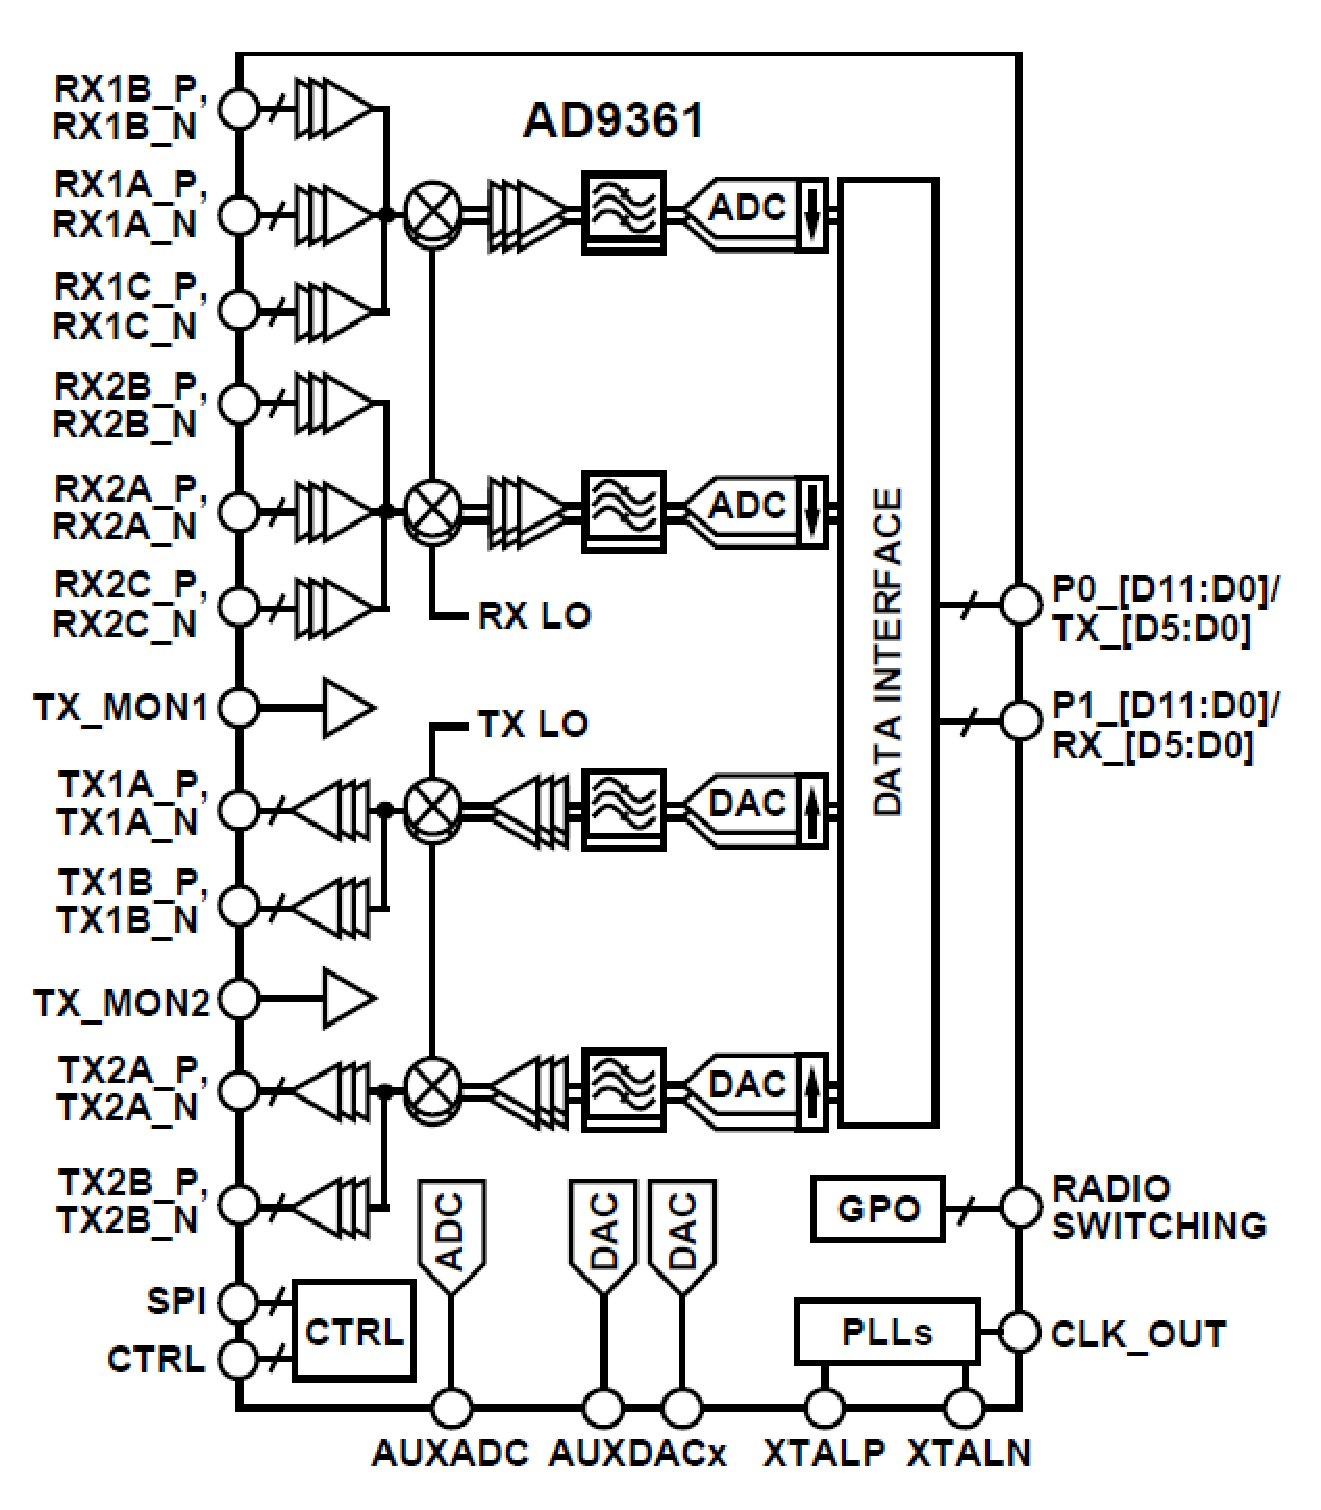
\includegraphics[width=0.65\textwidth]{./figures/ad9361_functional_diagram}
    \caption{ Image of the Setup Hardware
    \label{fig:setup}}
\end{figure}

%foto diagrama de blocos
\begin{figure}[htbp]
    \centering
    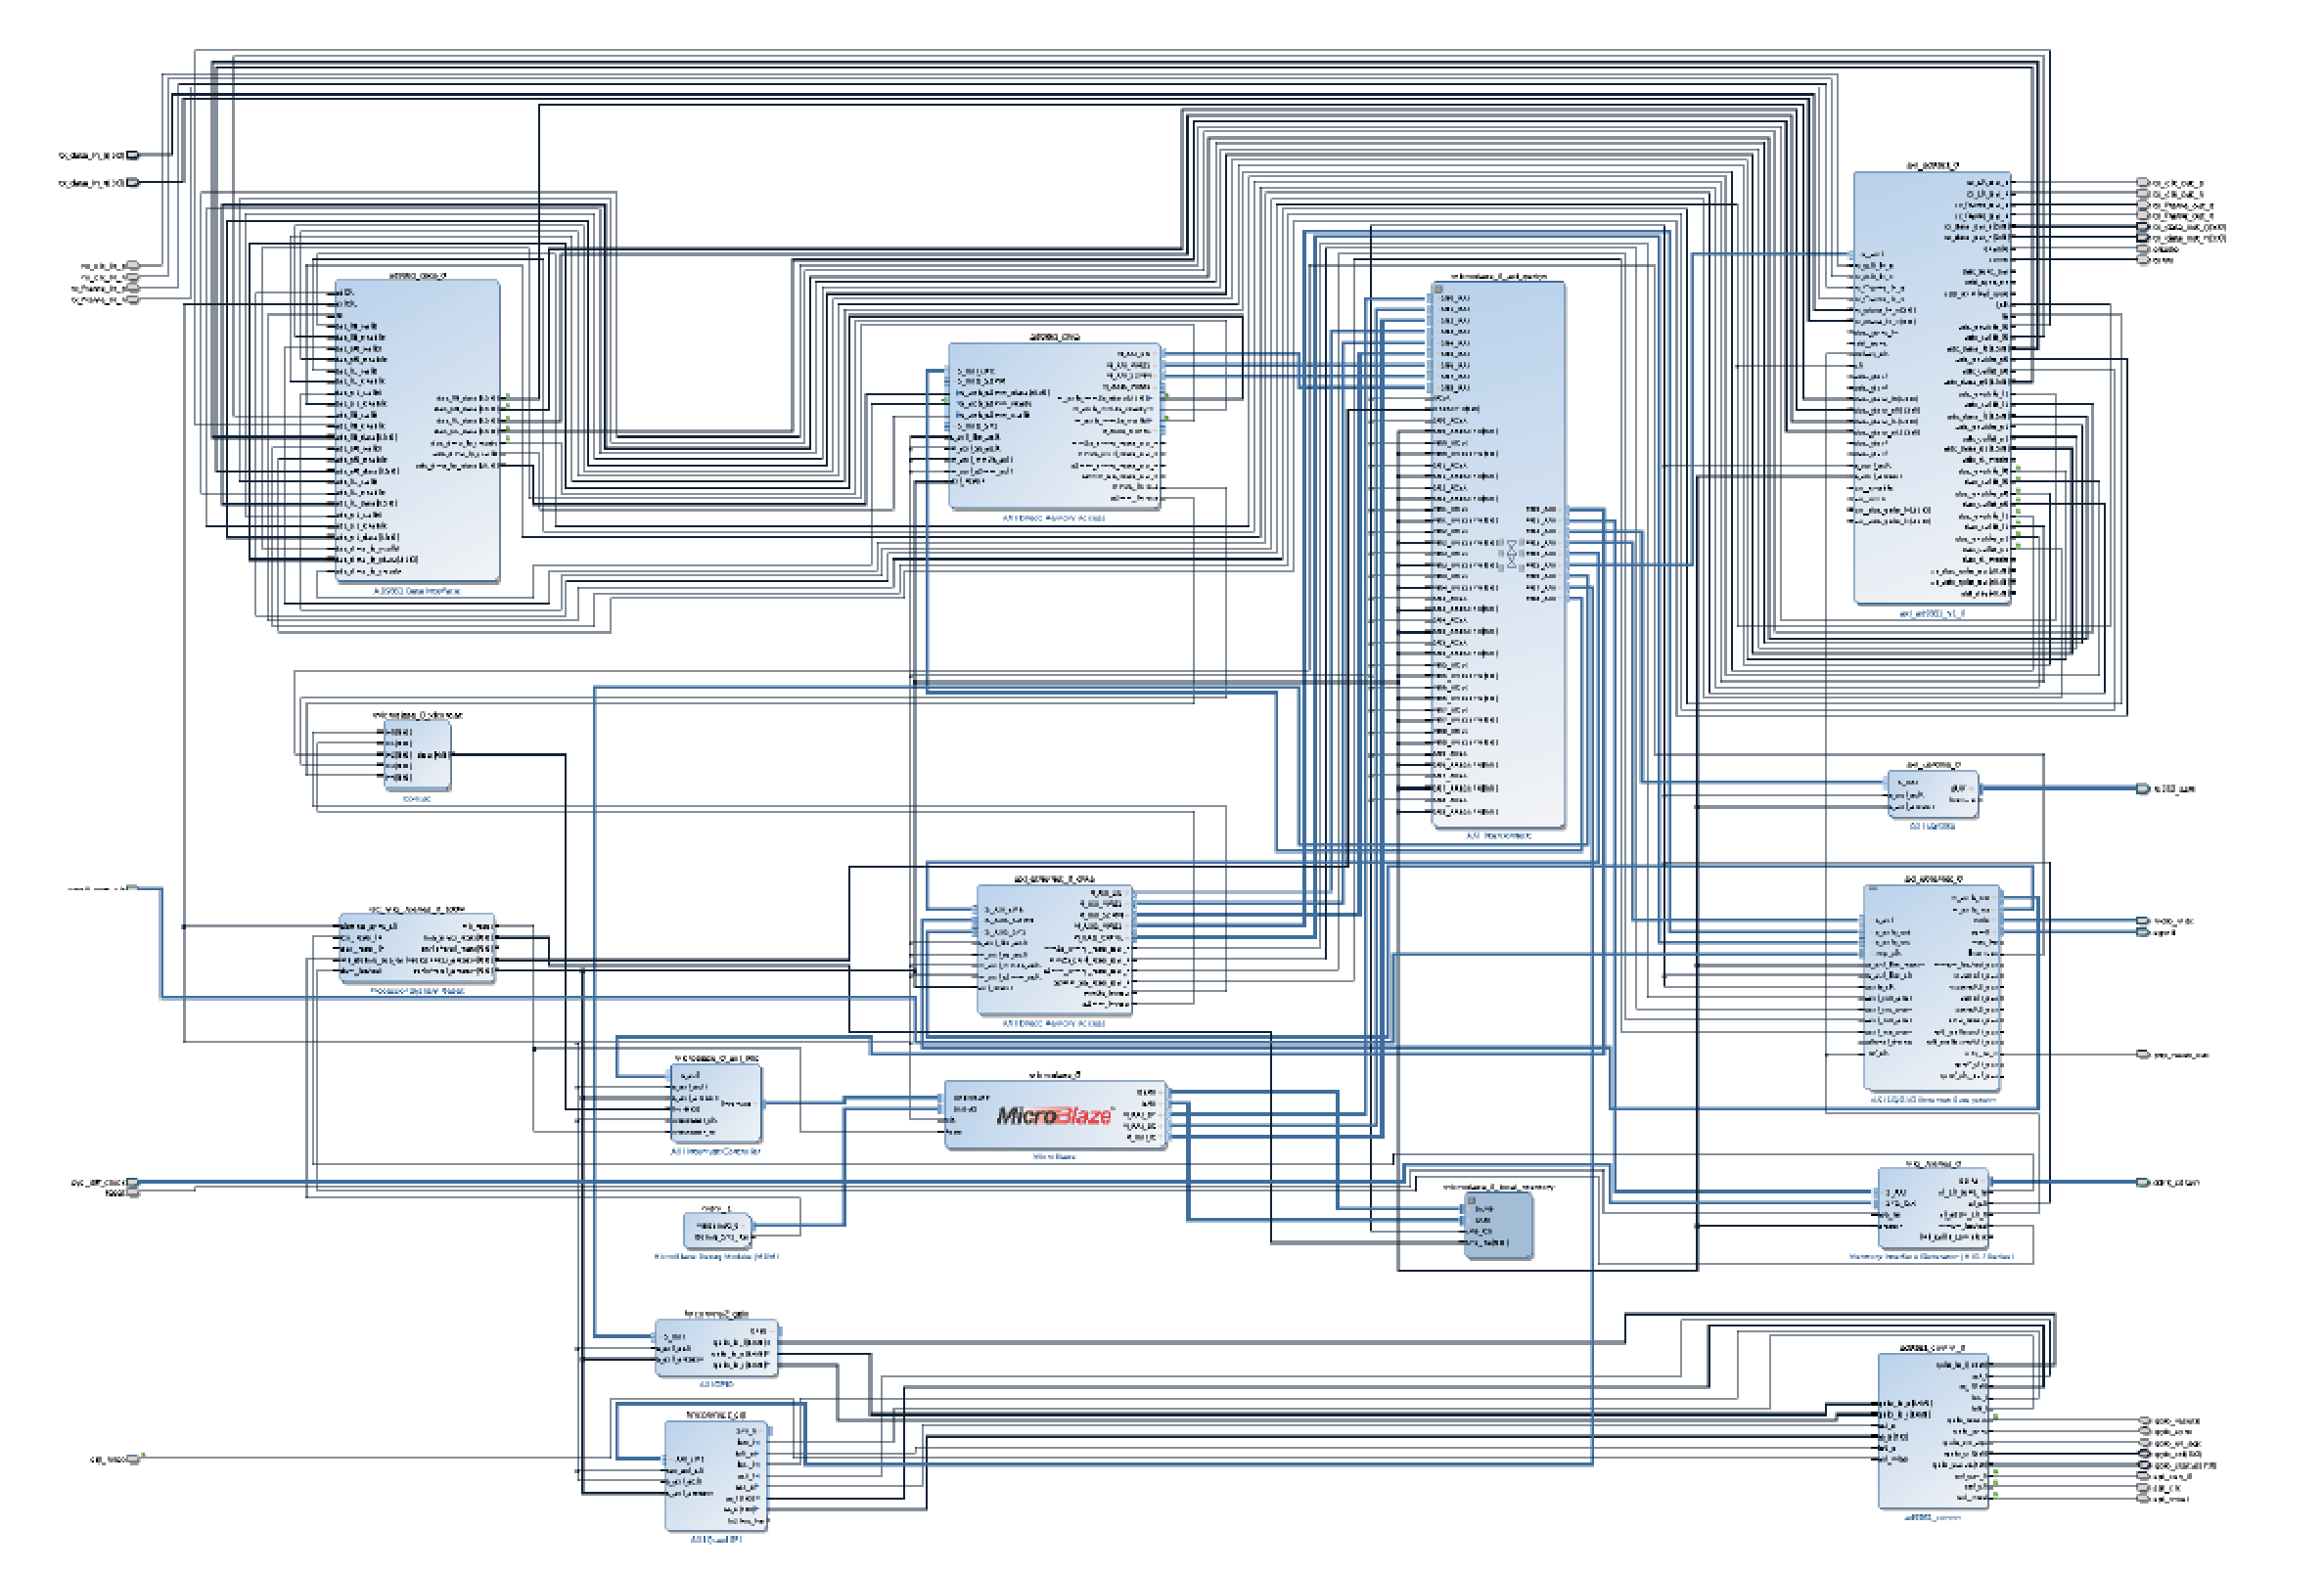
\includegraphics[width=0.95\textwidth]{./figures/setup_bd}
    \caption{ Image of the Setup Block diagram
    \label{fig:setupbd}}
\end{figure}

\newpage

\section{Preliminary Tests}
\label{result:conf}

The preliminary tests were focusing on initializing and communication between FPGA
and the FMComms2 board, in the previous chapter the steps of setting up communication
and control interface were described, and it describes also how this interface works
and how a block was made to implement such, in short it was needed to set up SPI and GPIO
modules and make the right input and output ports specified in \ref{subs:controlif} and
after the initialization and callibration is finished, it is possible to observ the
carrier wave centralized at the frequency 2.4 Ghz.

To generate the outputs two analyzers were used, one oscilloscope and one spectrum analyzer,
both analyzers outputs can be seen in the figures below:

%spectrum analyser image
\begin{figure}[htbp]
    \centering
    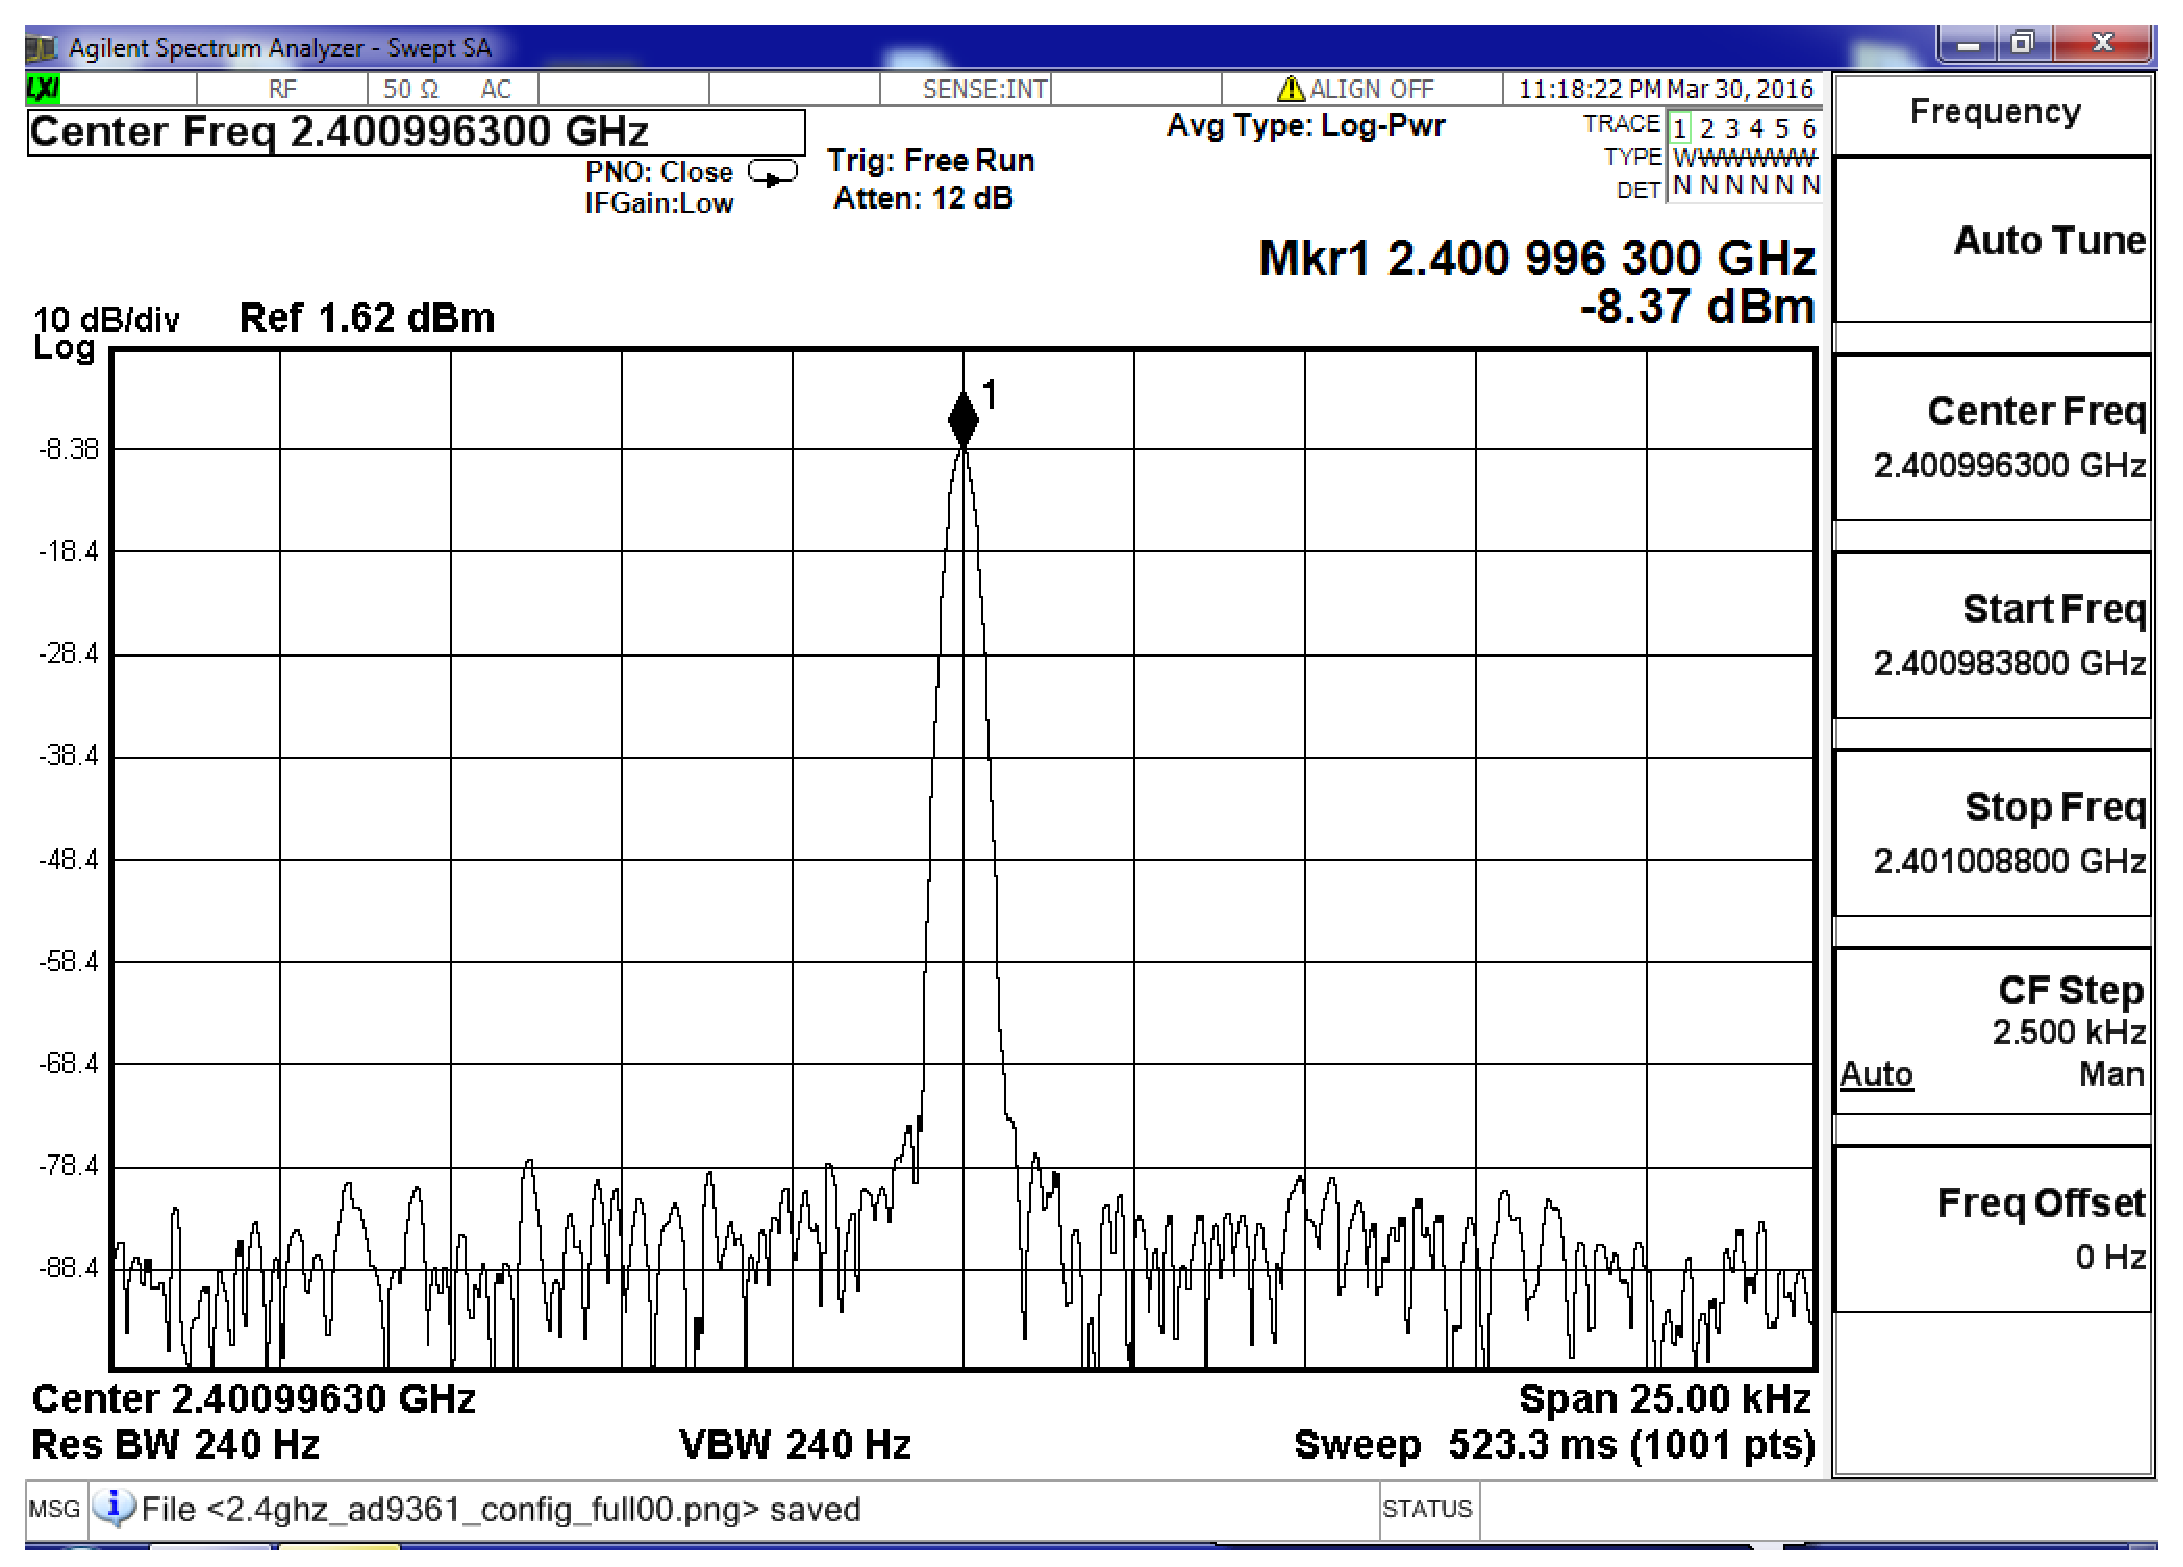
\includegraphics[width=0.85\textwidth]{./figures/spectrum_init}
    \caption{ Spectrum Analyzer Screen
    \label{fig:spec}}
\end{figure}

%initialization
\begin{figure}[htbp]
    \centering
    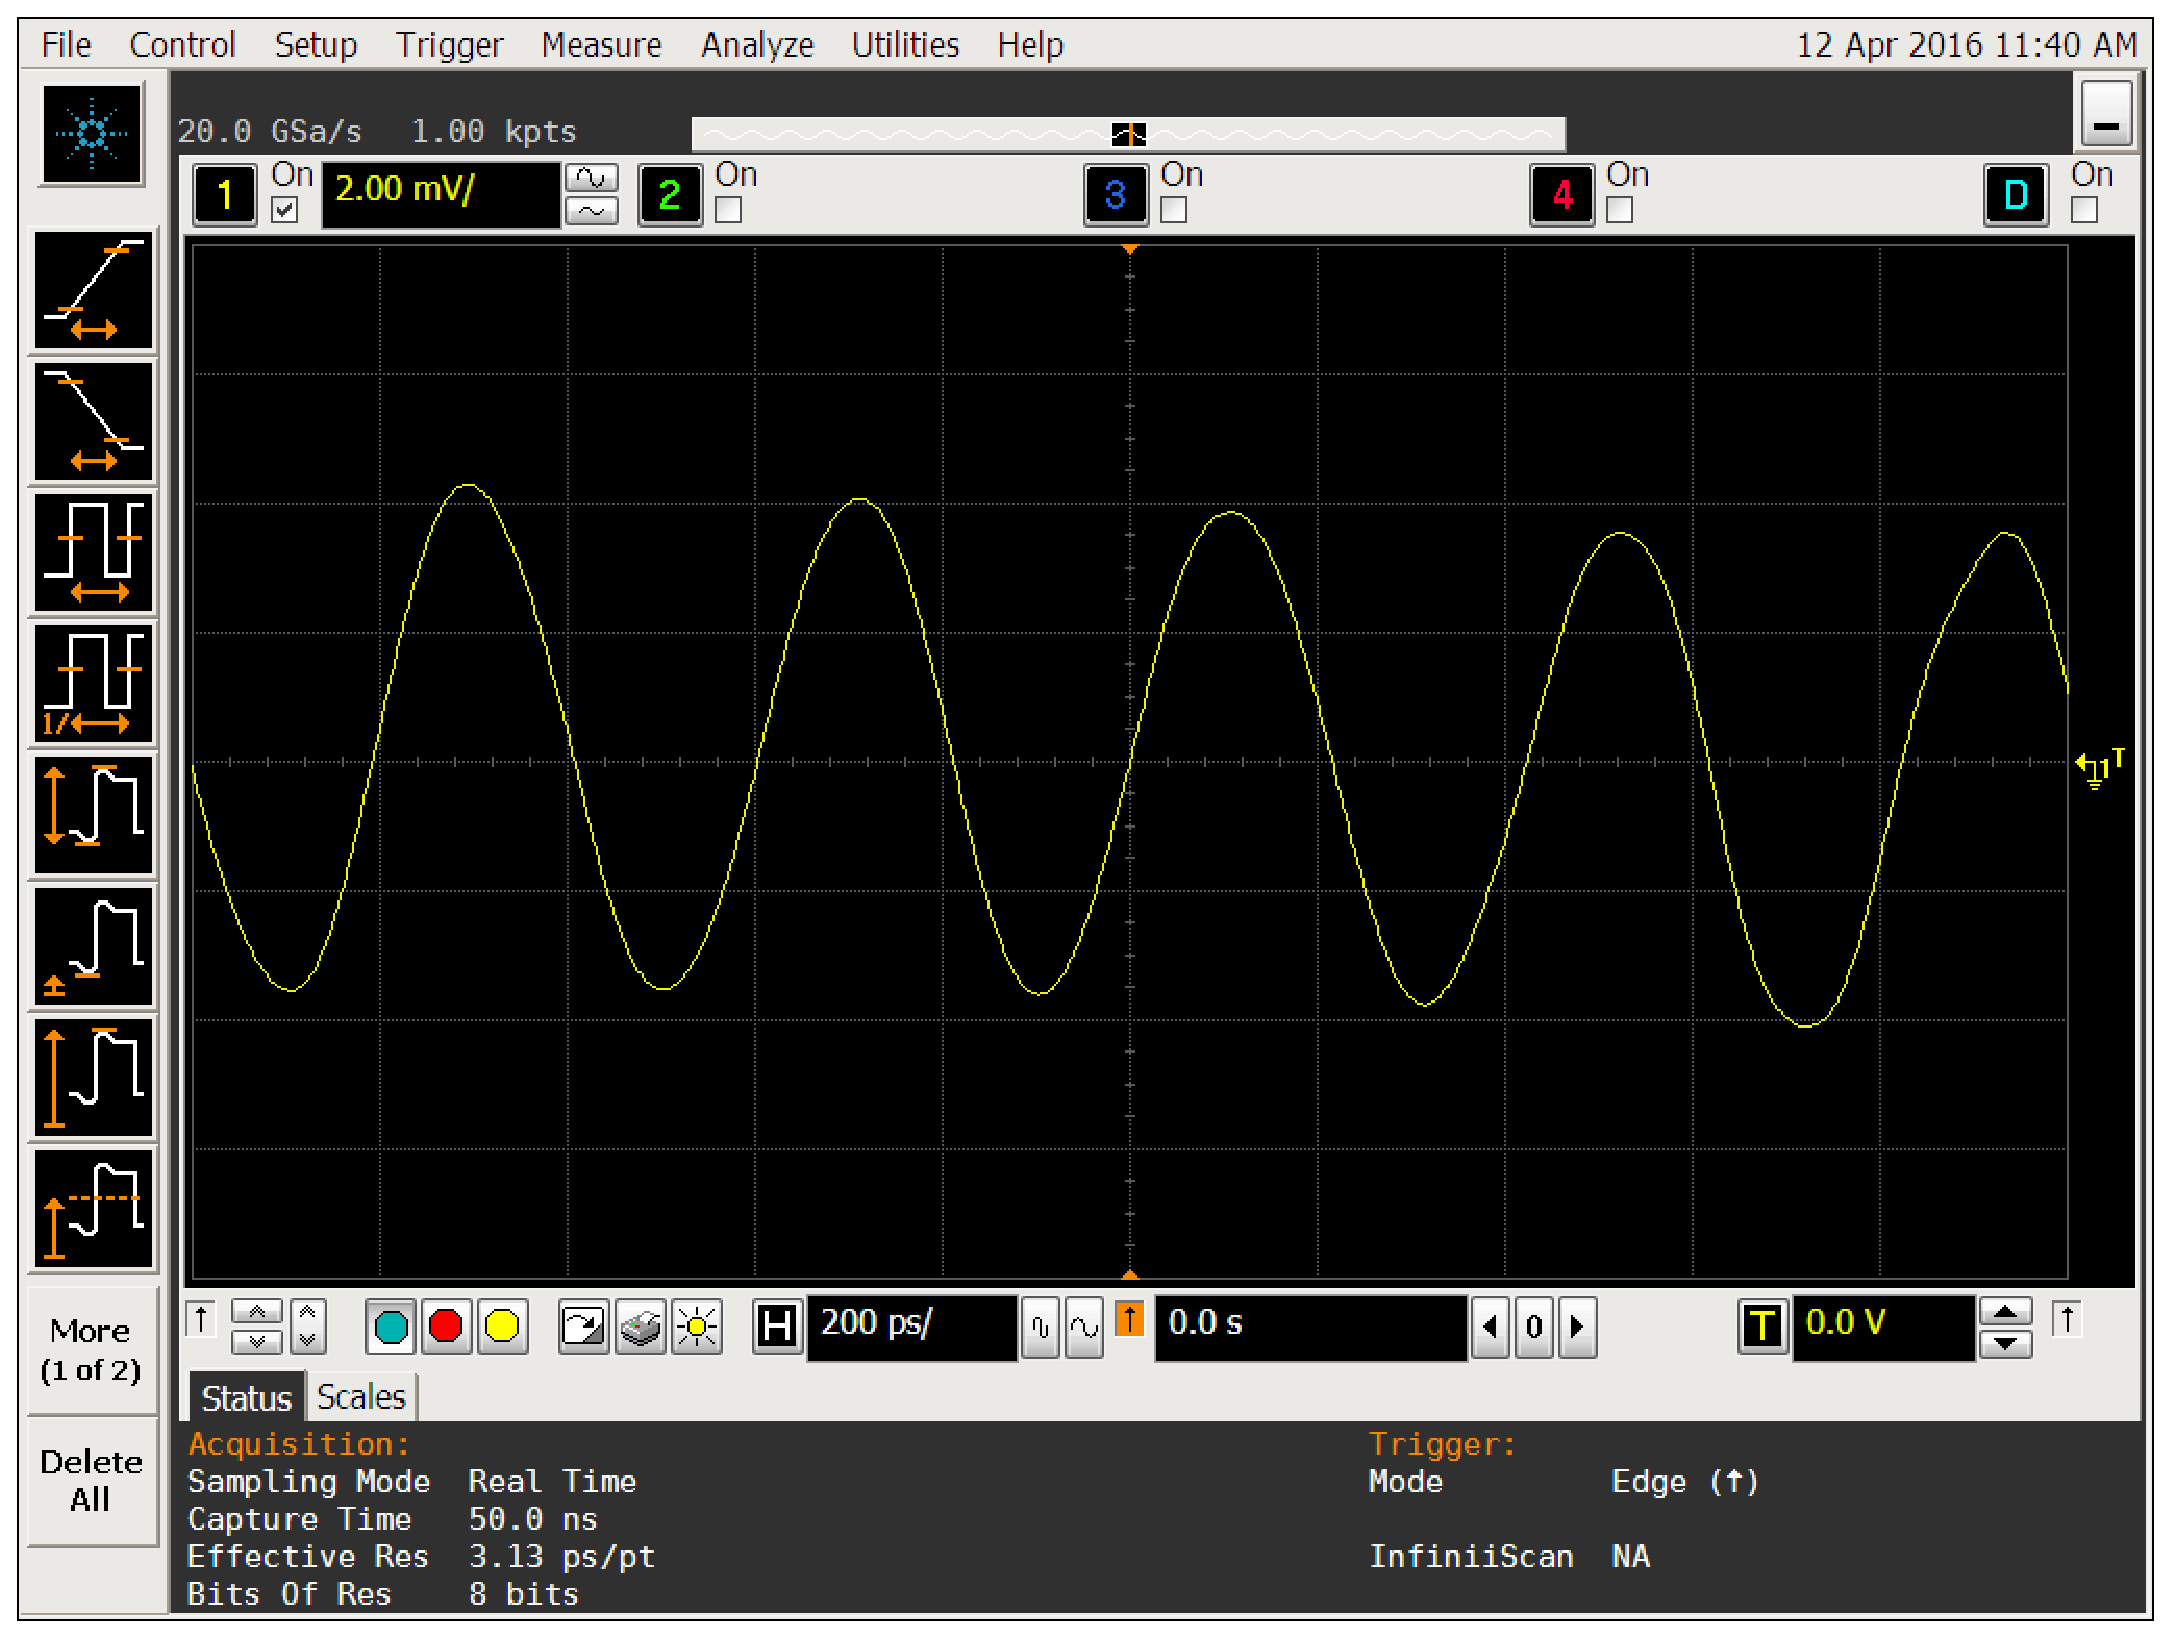
\includegraphics[width=0.85\textwidth]{./figures/oscill_init}
    \caption{ Carrier Waveform after Initialization
    \label{fig:oscillinit}}
\end{figure}

%digital tune
\begin{figure}[htbp]
    \centering
    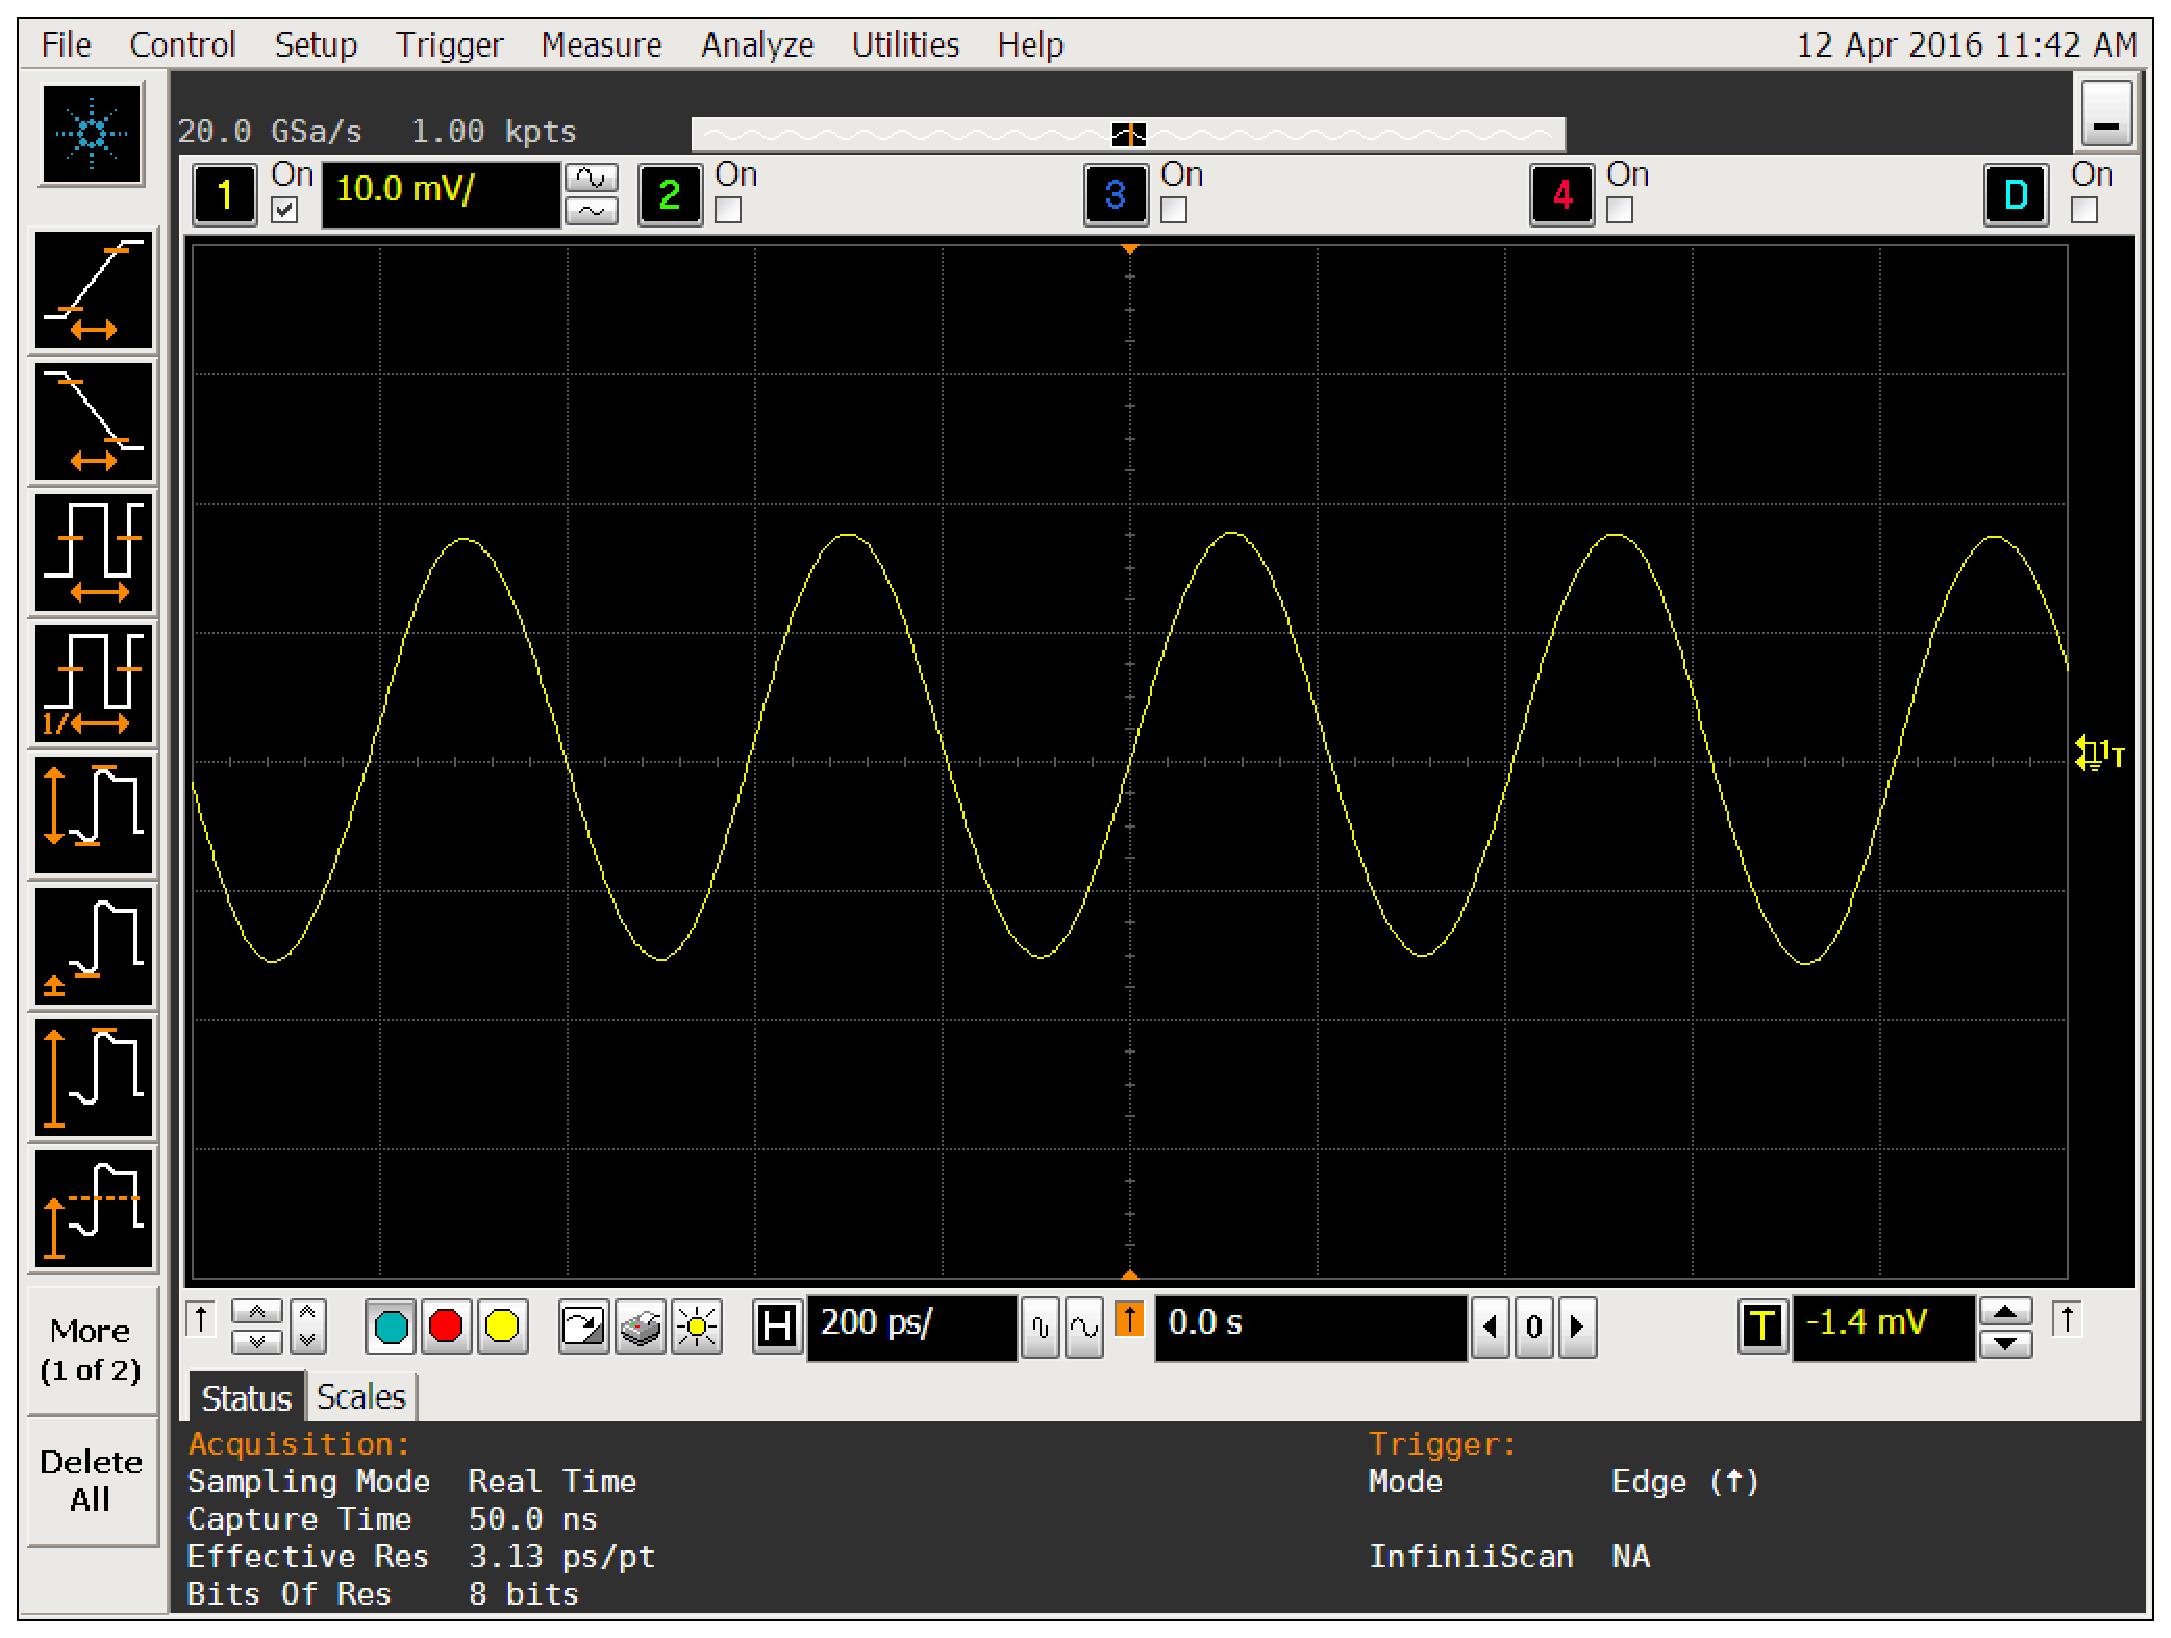
\includegraphics[width=0.85\textwidth]{./figures/oscill_dig}
    \caption{ Carrier Waveform after Tunning Digital Interface
    \label{fig:oscilldig}}
\end{figure}

%freq
\begin{figure}[htbp]
    \centering
    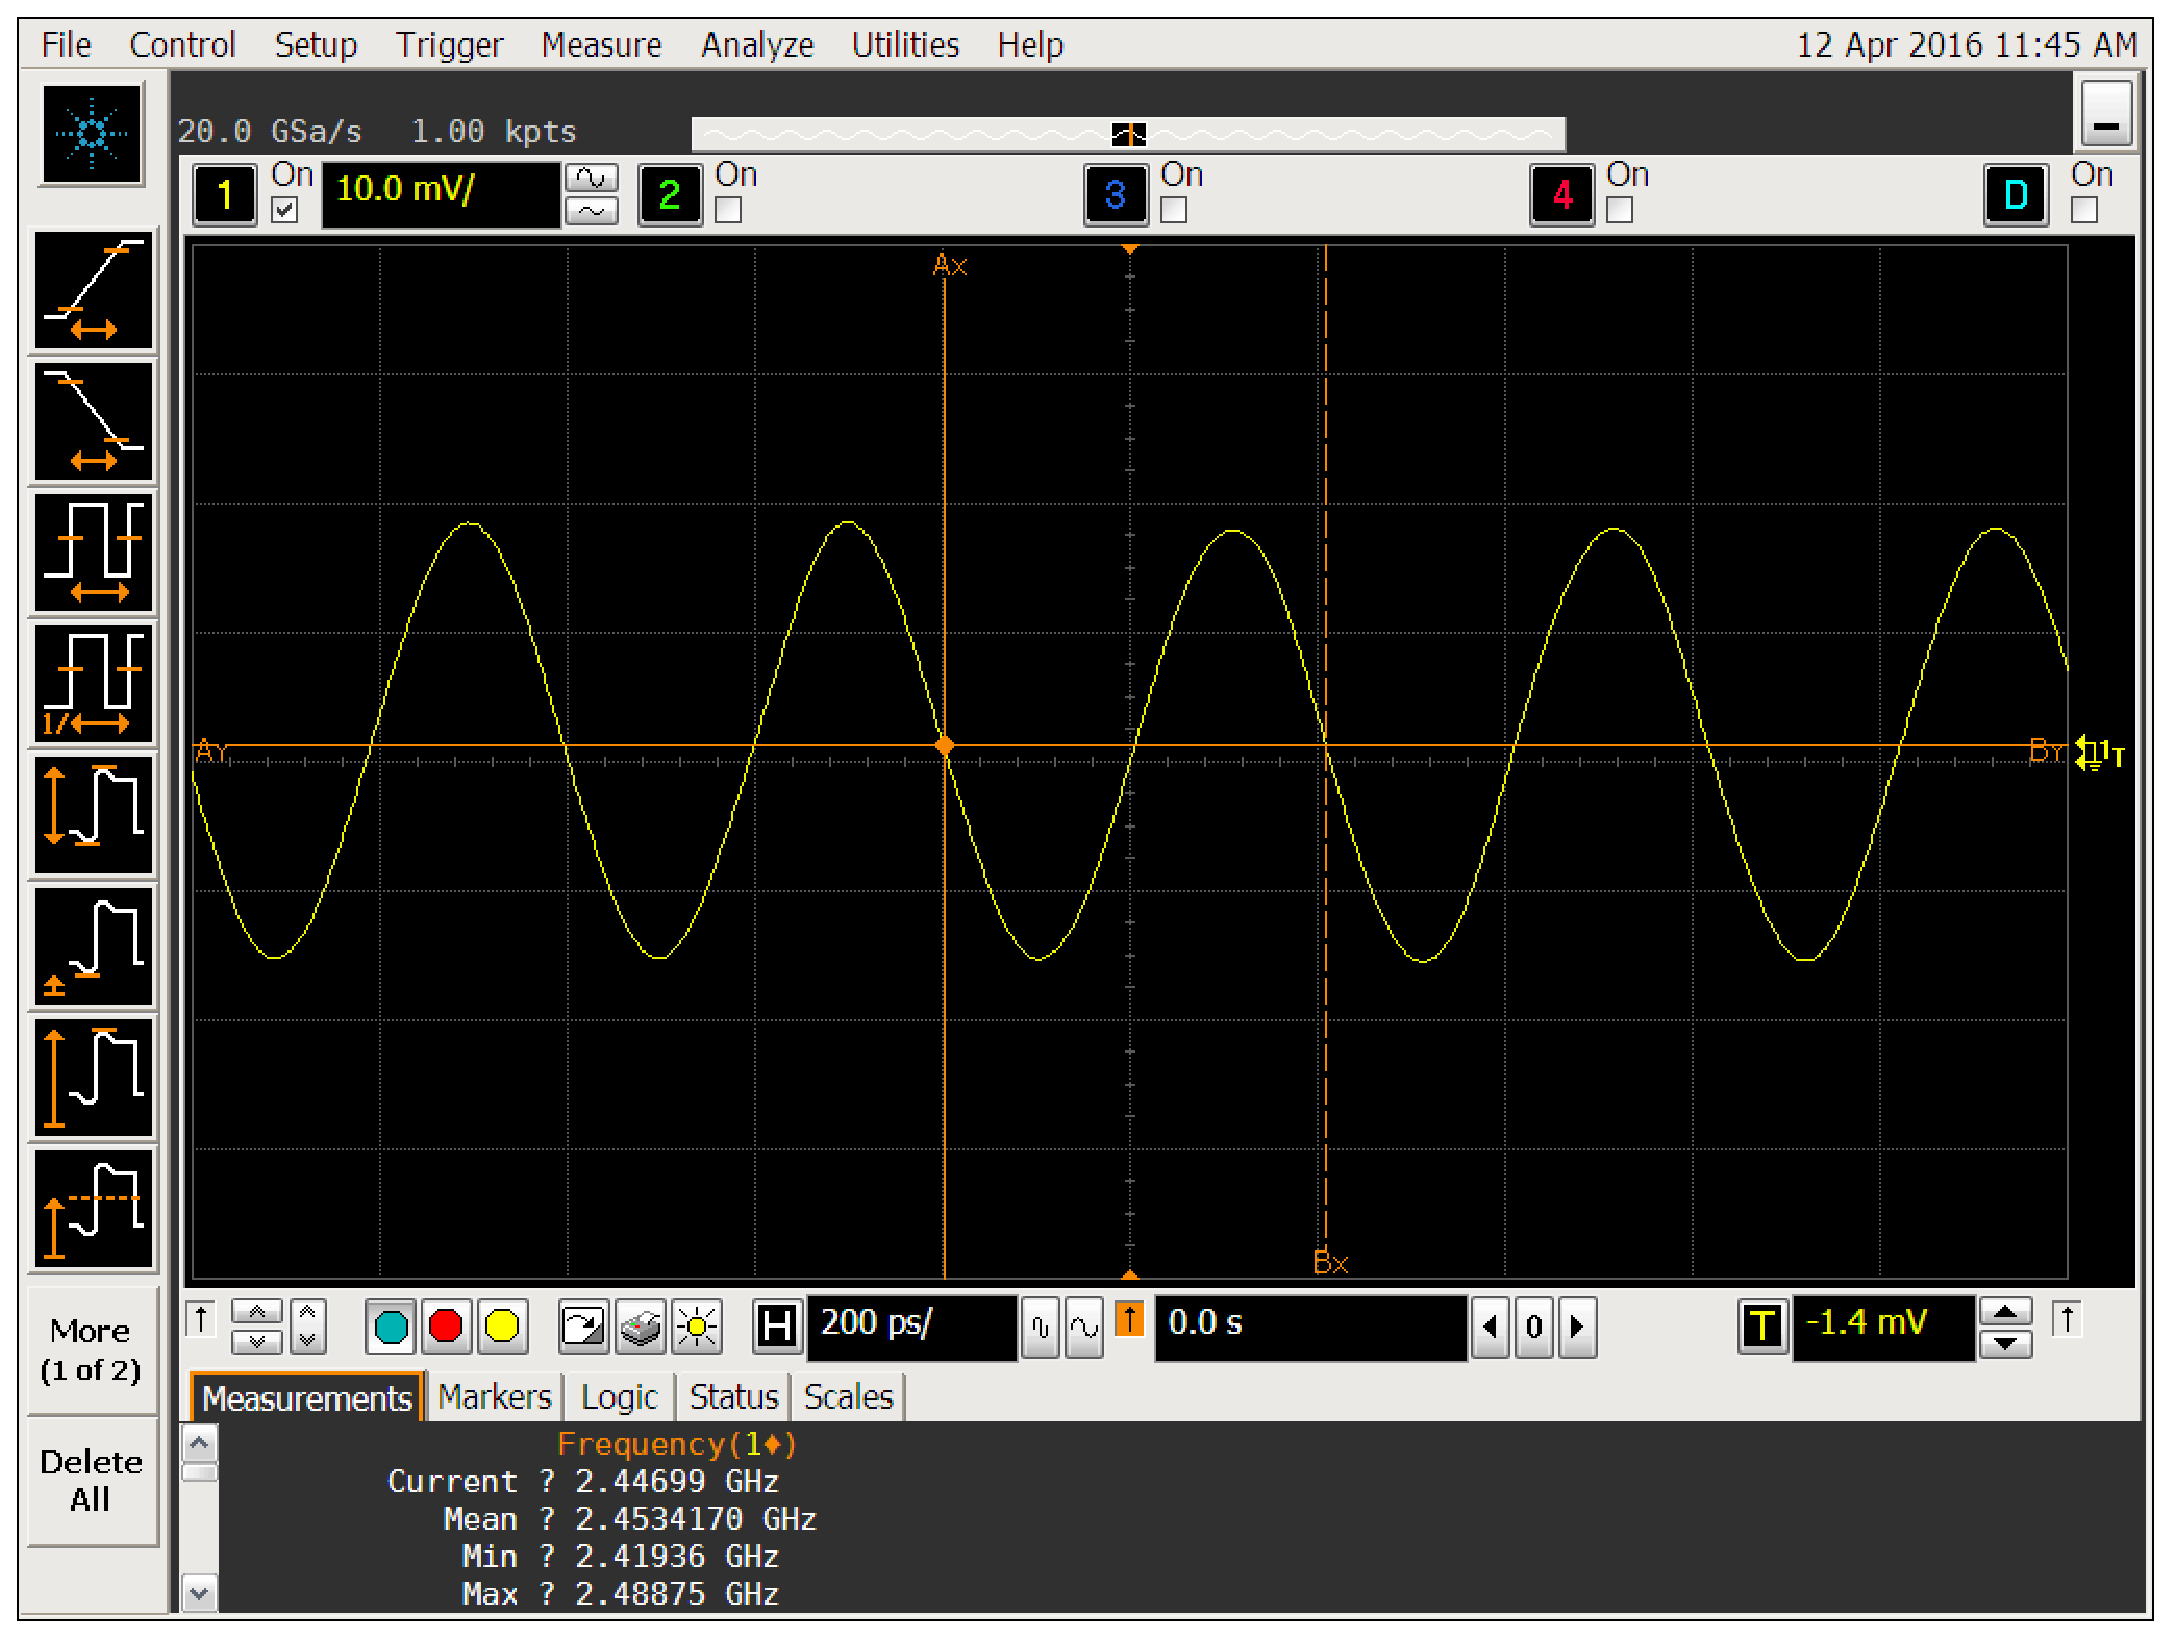
\includegraphics[width=0.85\textwidth]{./figures/oscill_freq}
    \caption{ Carrier Waveform with Frequency Measure
    \label{fig:oscillfreq}}
\end{figure}

%fft config
\begin{figure}[htbp]
    \centering
    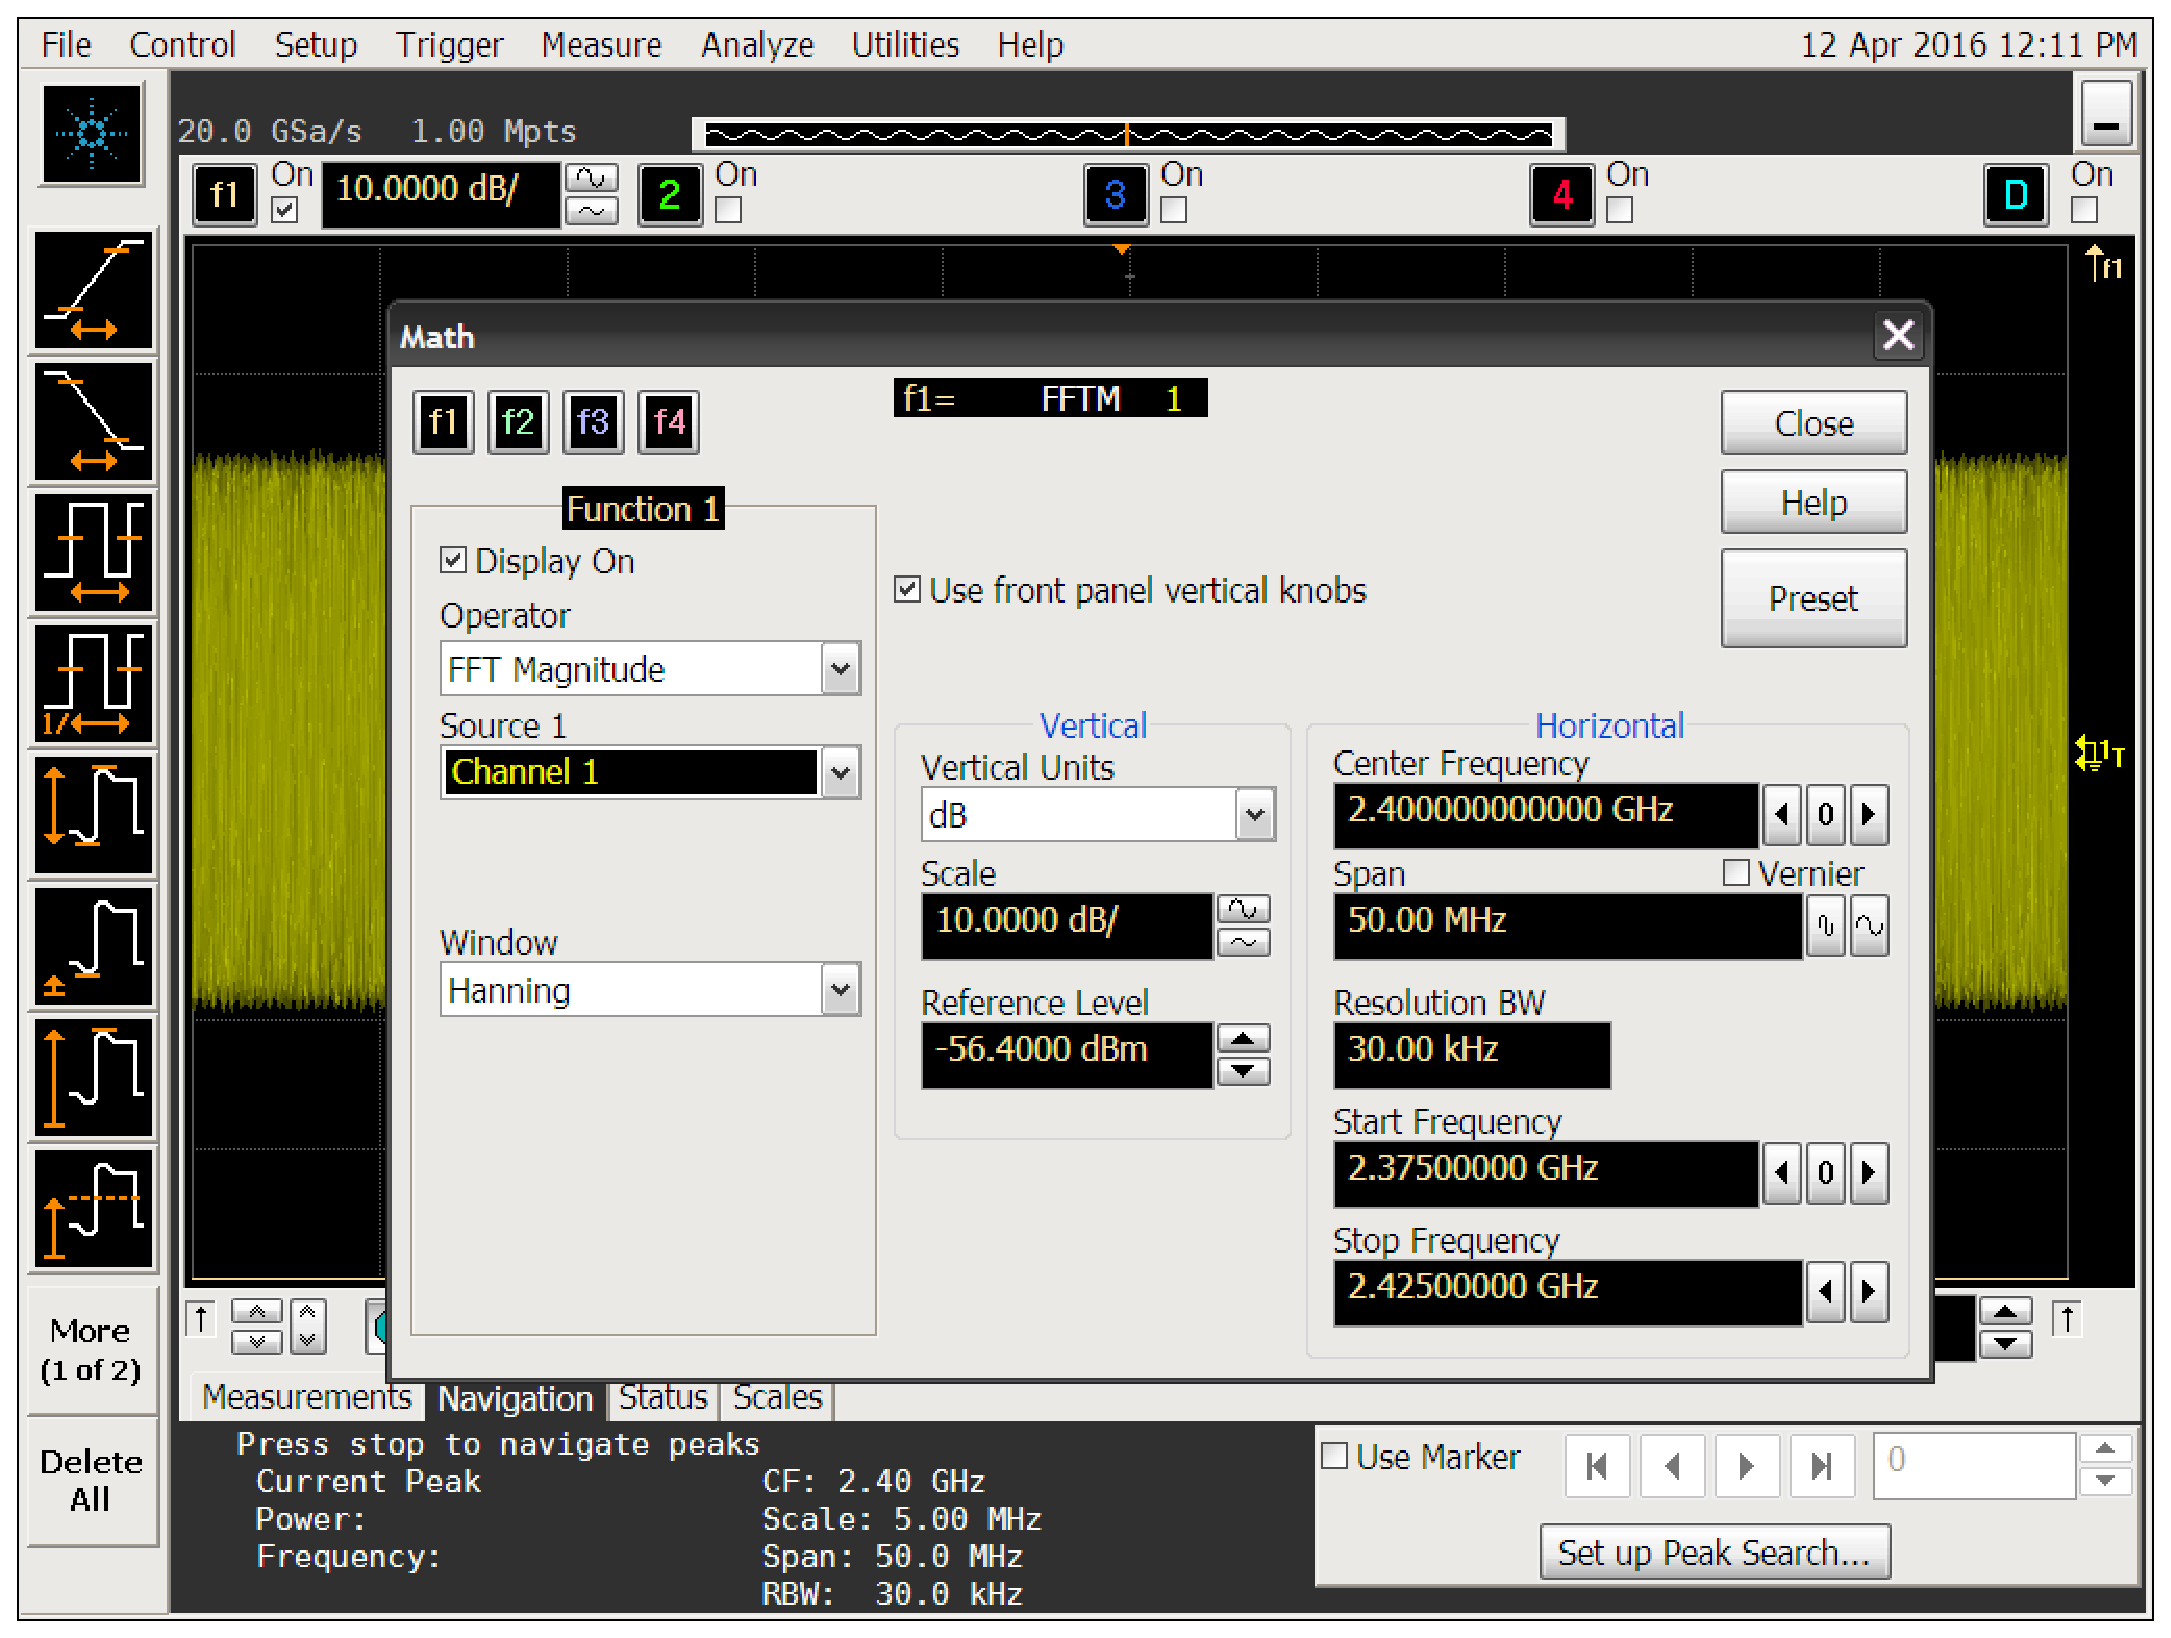
\includegraphics[width=0.85\textwidth]{./figures/oscill_fftcf}
    \caption{ FFT Configuration Parameters
    \label{fig:oscillfftcf}}
\end{figure}

%wave + fft
\begin{figure}[htbp]
    \centering
    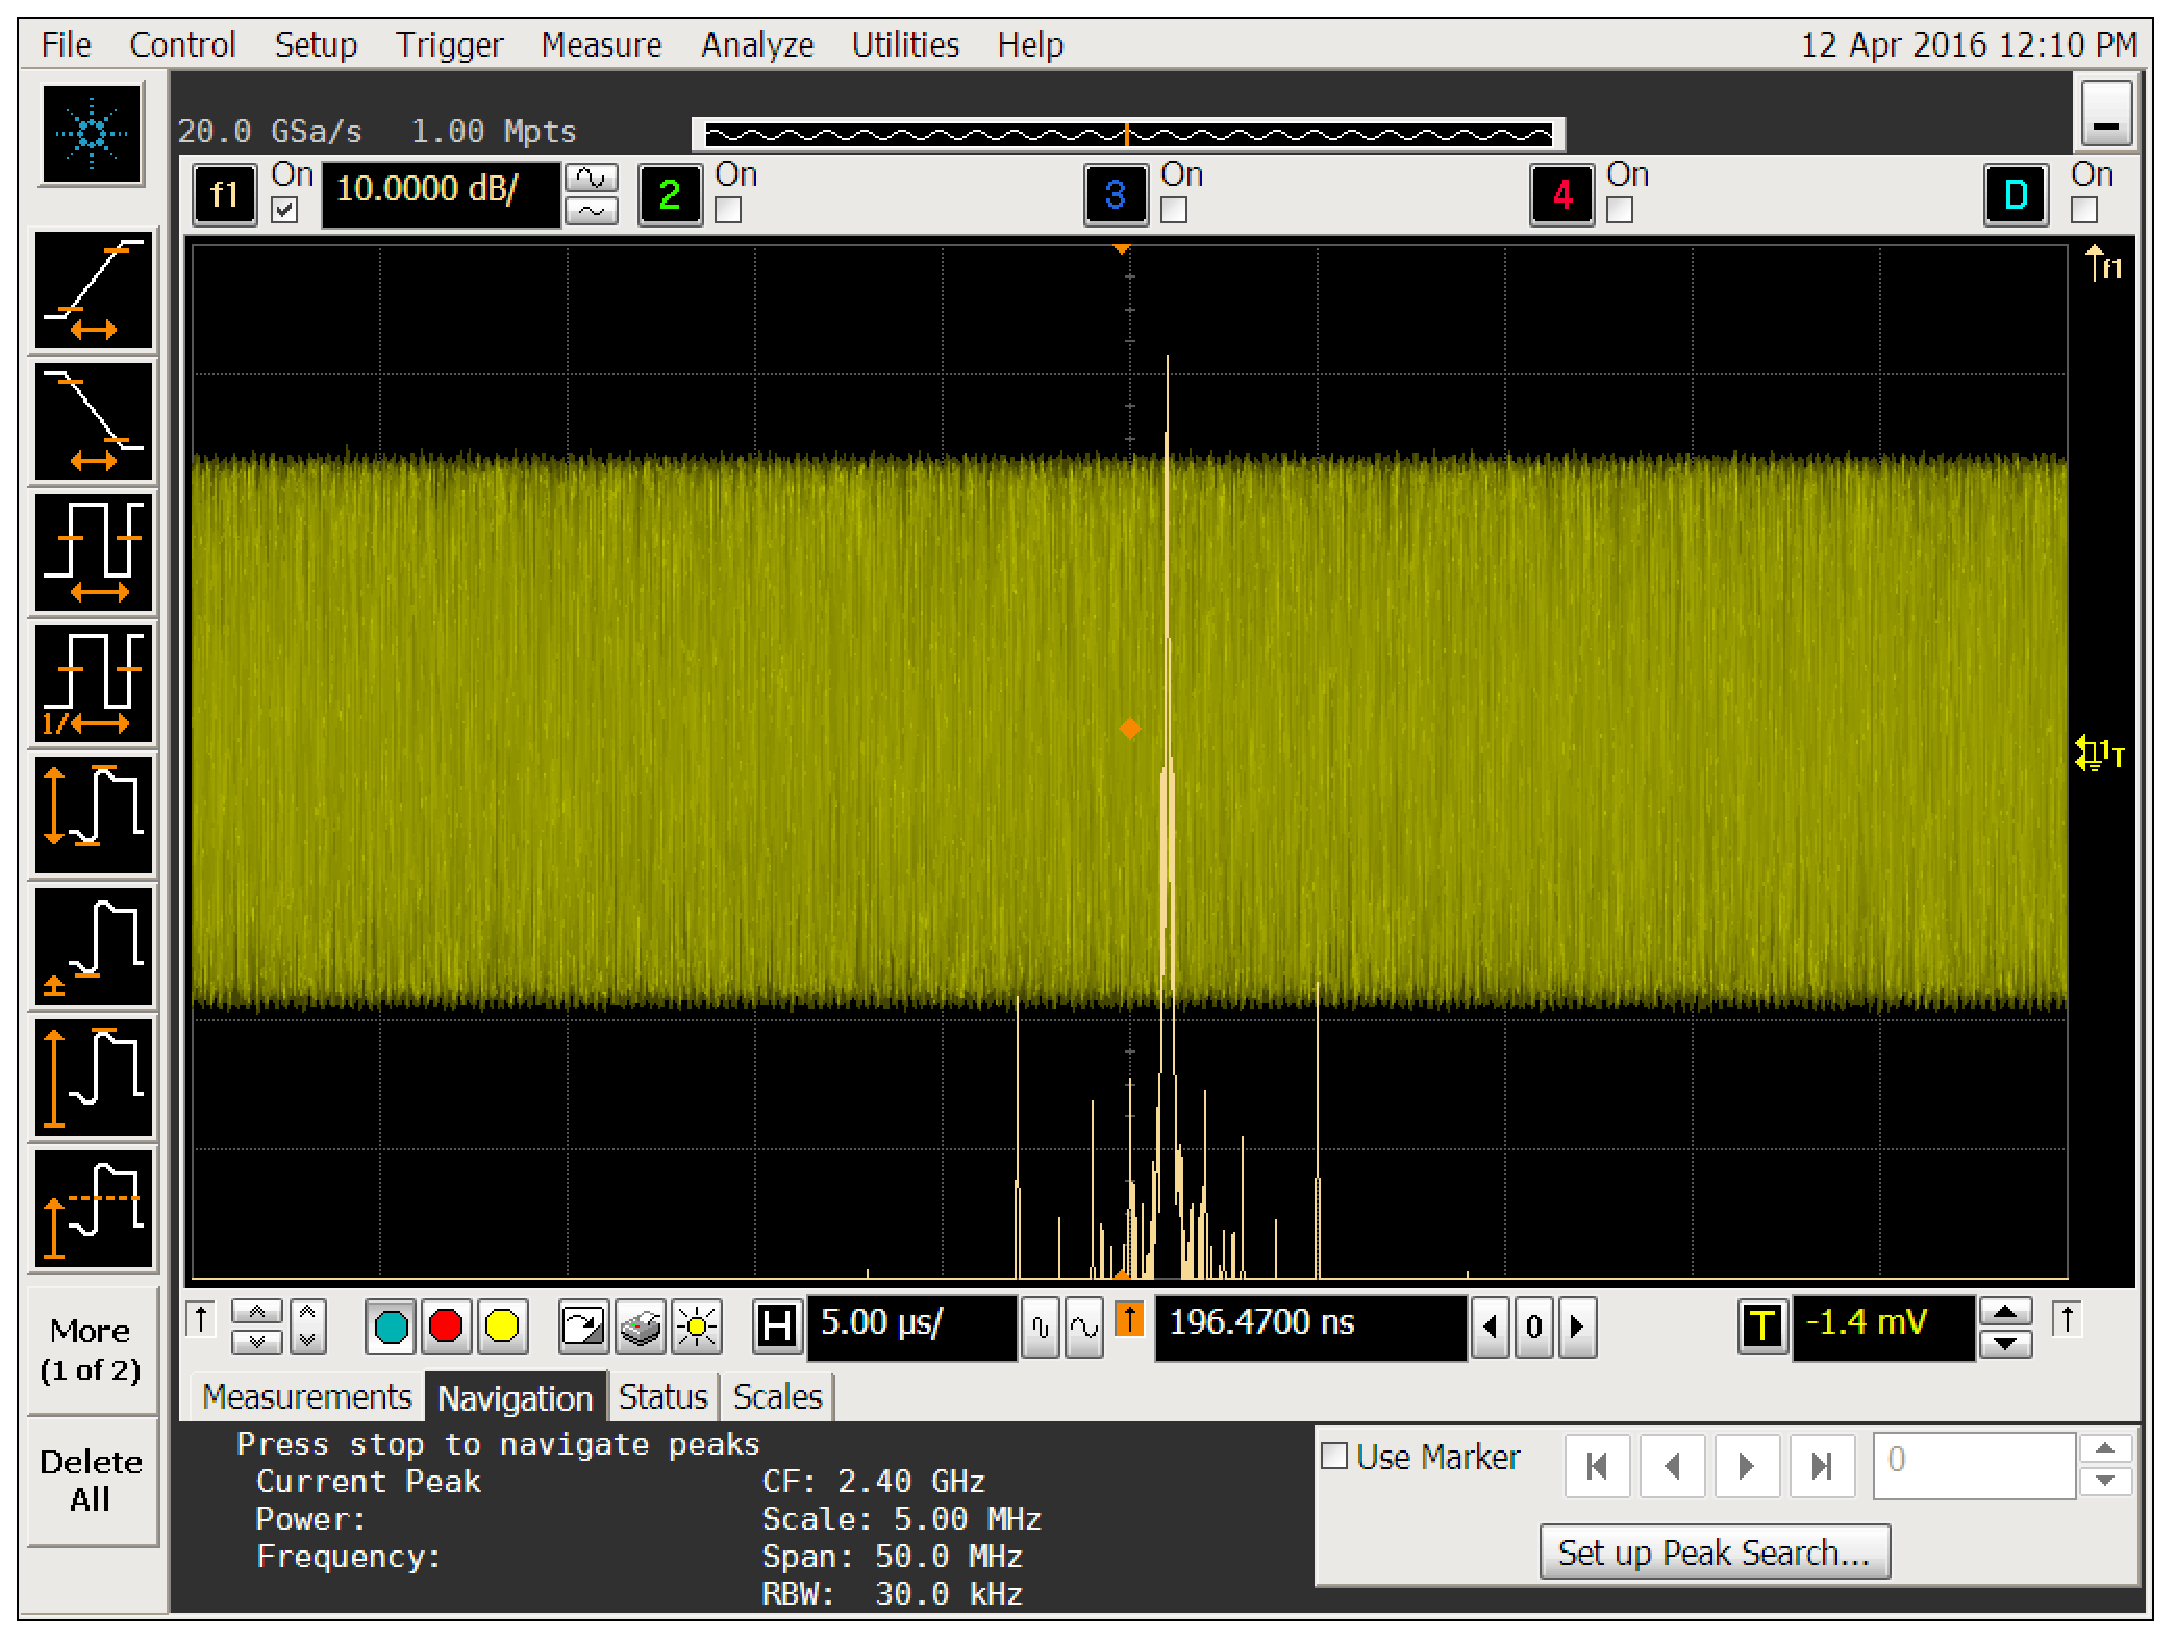
\includegraphics[width=0.85\textwidth]{./figures/oscill_fft}
    \caption{ FFT and Carrier Waveform
    \label{fig:oscillfft}}
\end{figure}

\section{Simulation}

An important step in HDL development is the logic simulation of the circuit,
through this simulation it is possible to watch every port and be able to
understand the block behavior, thus correcting any problem or misbehavior.\\

\subsection{Transmit (DAC) Interface Simulation}

The simulation of the transmit interface, which interfaces the FPGA with DAC was
made in three steps, since the interface is composed by two blocks, there was
the need to simulate each block separately and after this simulate both blocks
connected and working together, in the figures \ref{fig:simdacdma},
\ref{fig:simdac} and \ref{fig:simtxif} it is possible to see the simulation
results and wave diagrams of the three steps.\\

\begin{figure}[htbp]
    \centering
    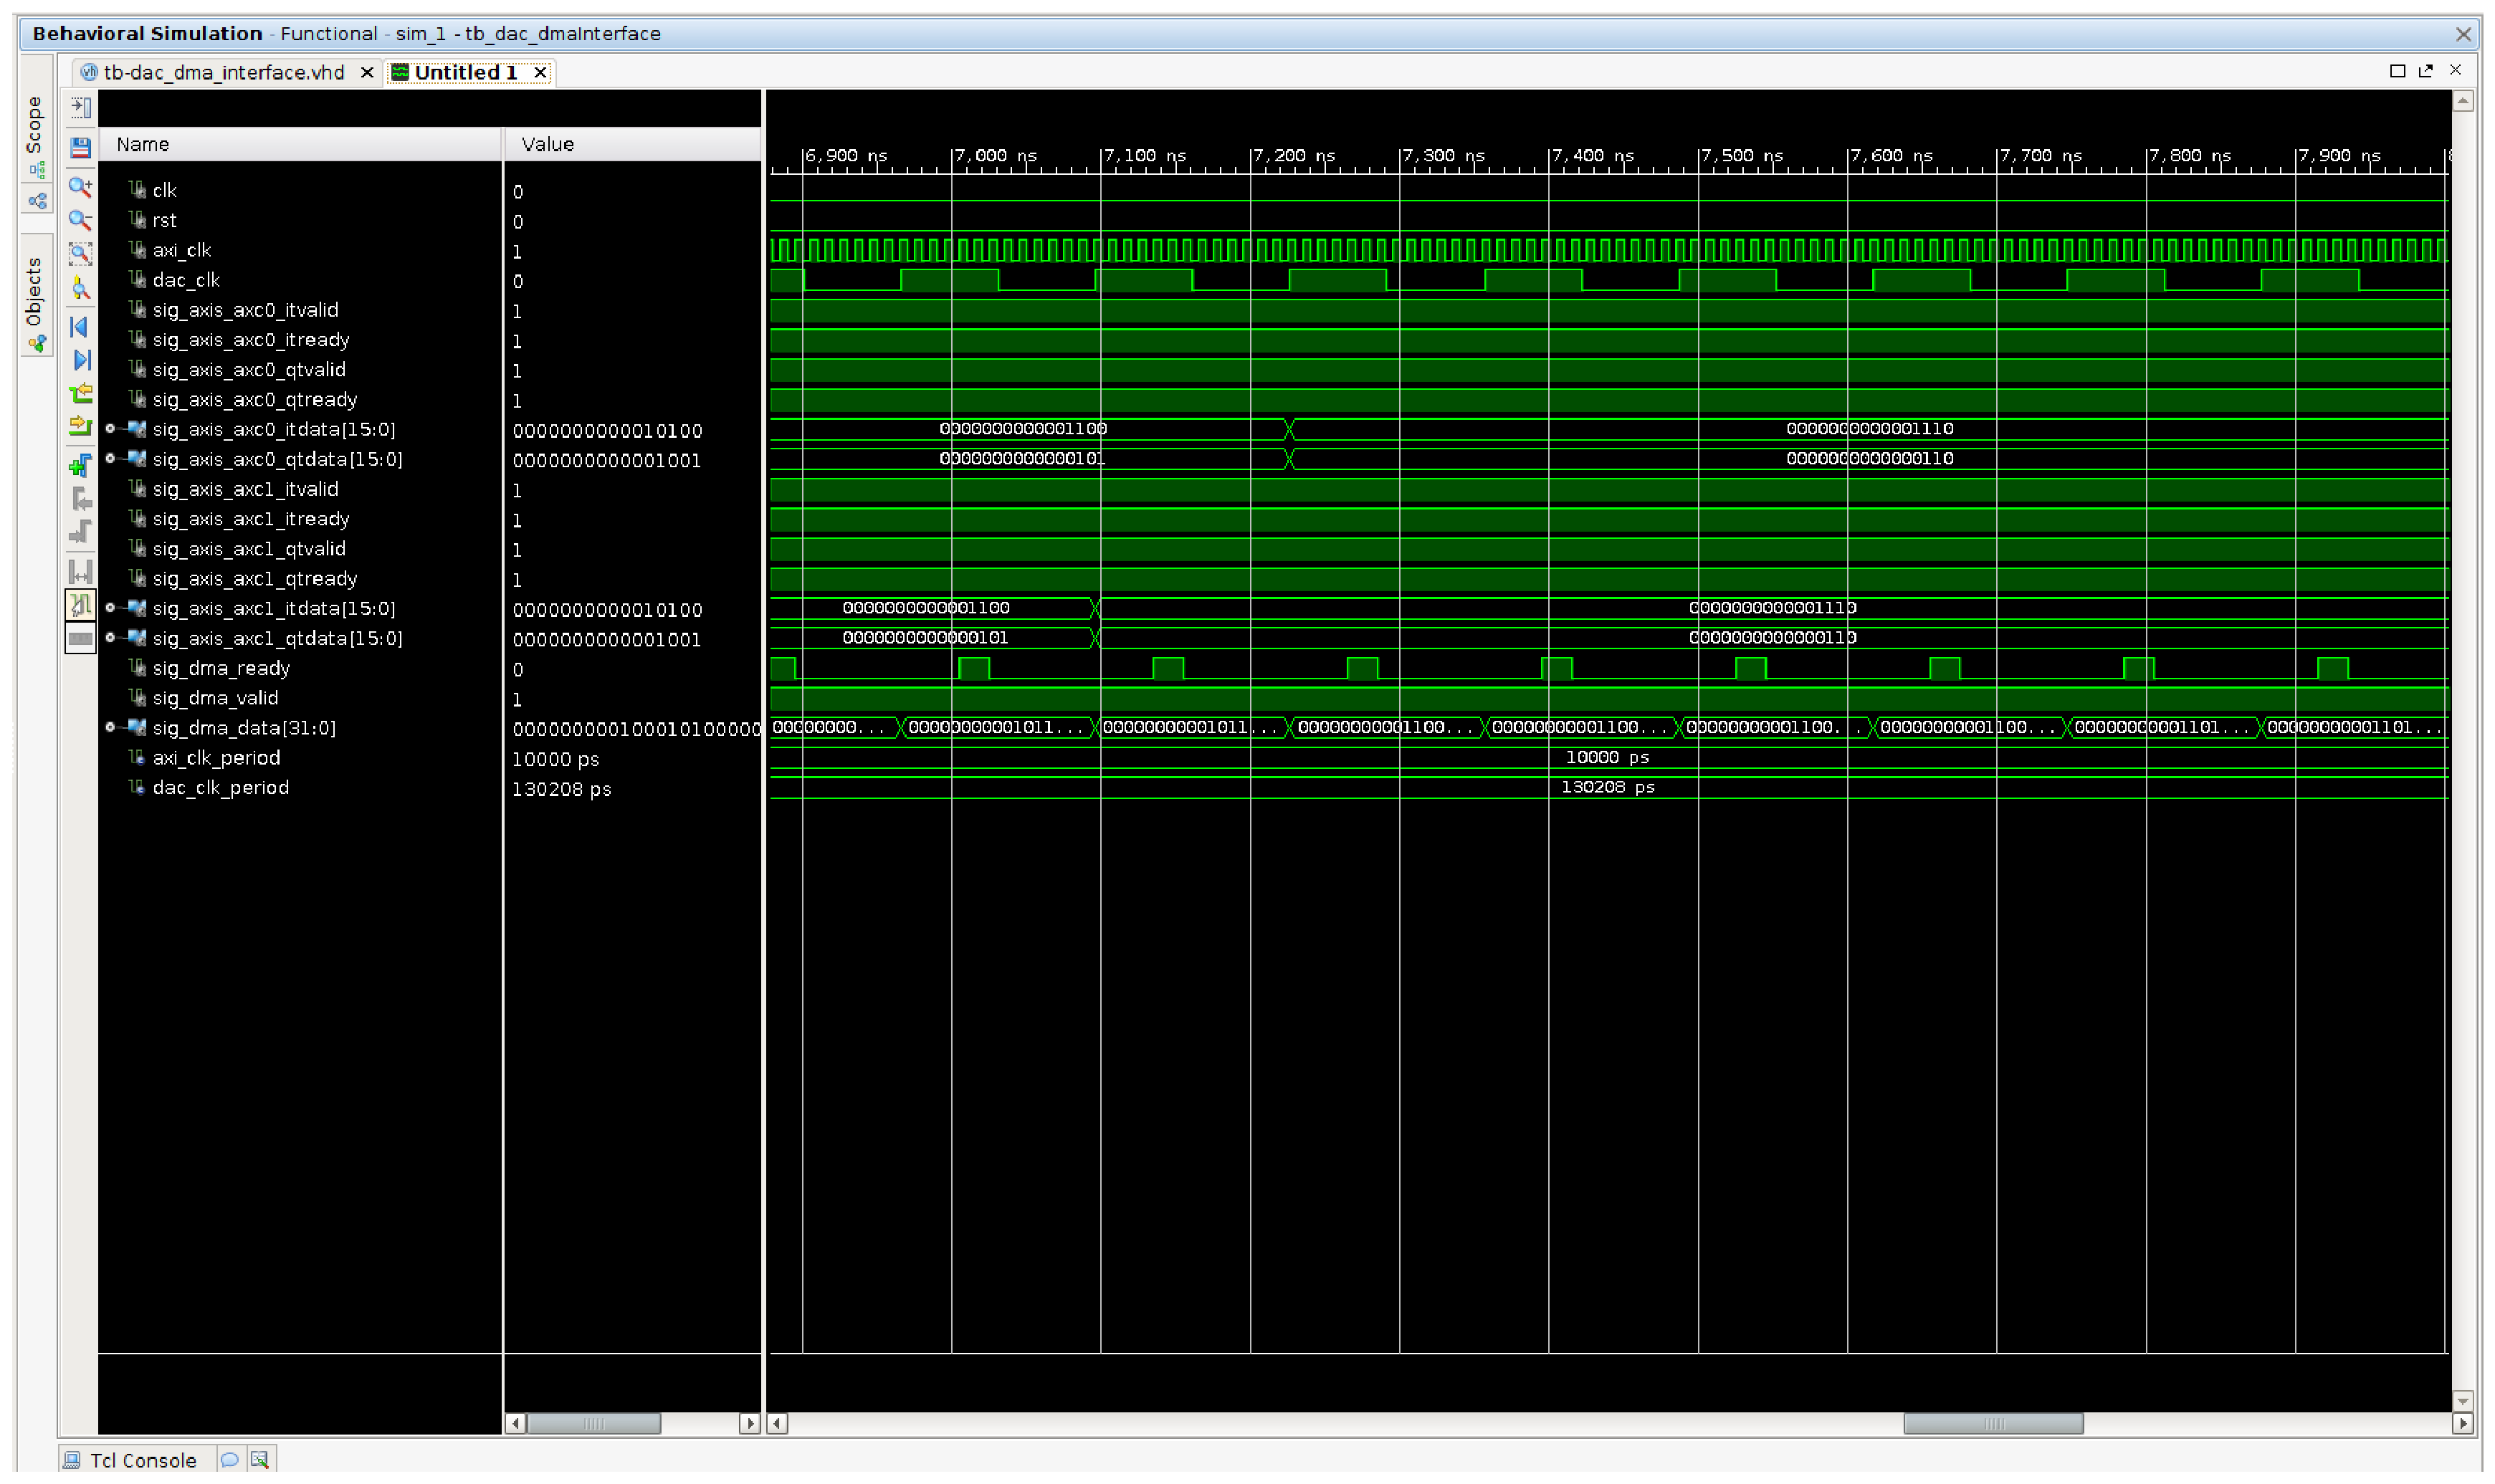
\includegraphics[width=0.95\textwidth]{./figures/dac_dmaInterface}
    \caption{ Step 1: DAC-DMA Interface Block Simulation
    \label{fig:simdacdma}}
\end{figure}

\begin{figure}[htbp]
    \centering
    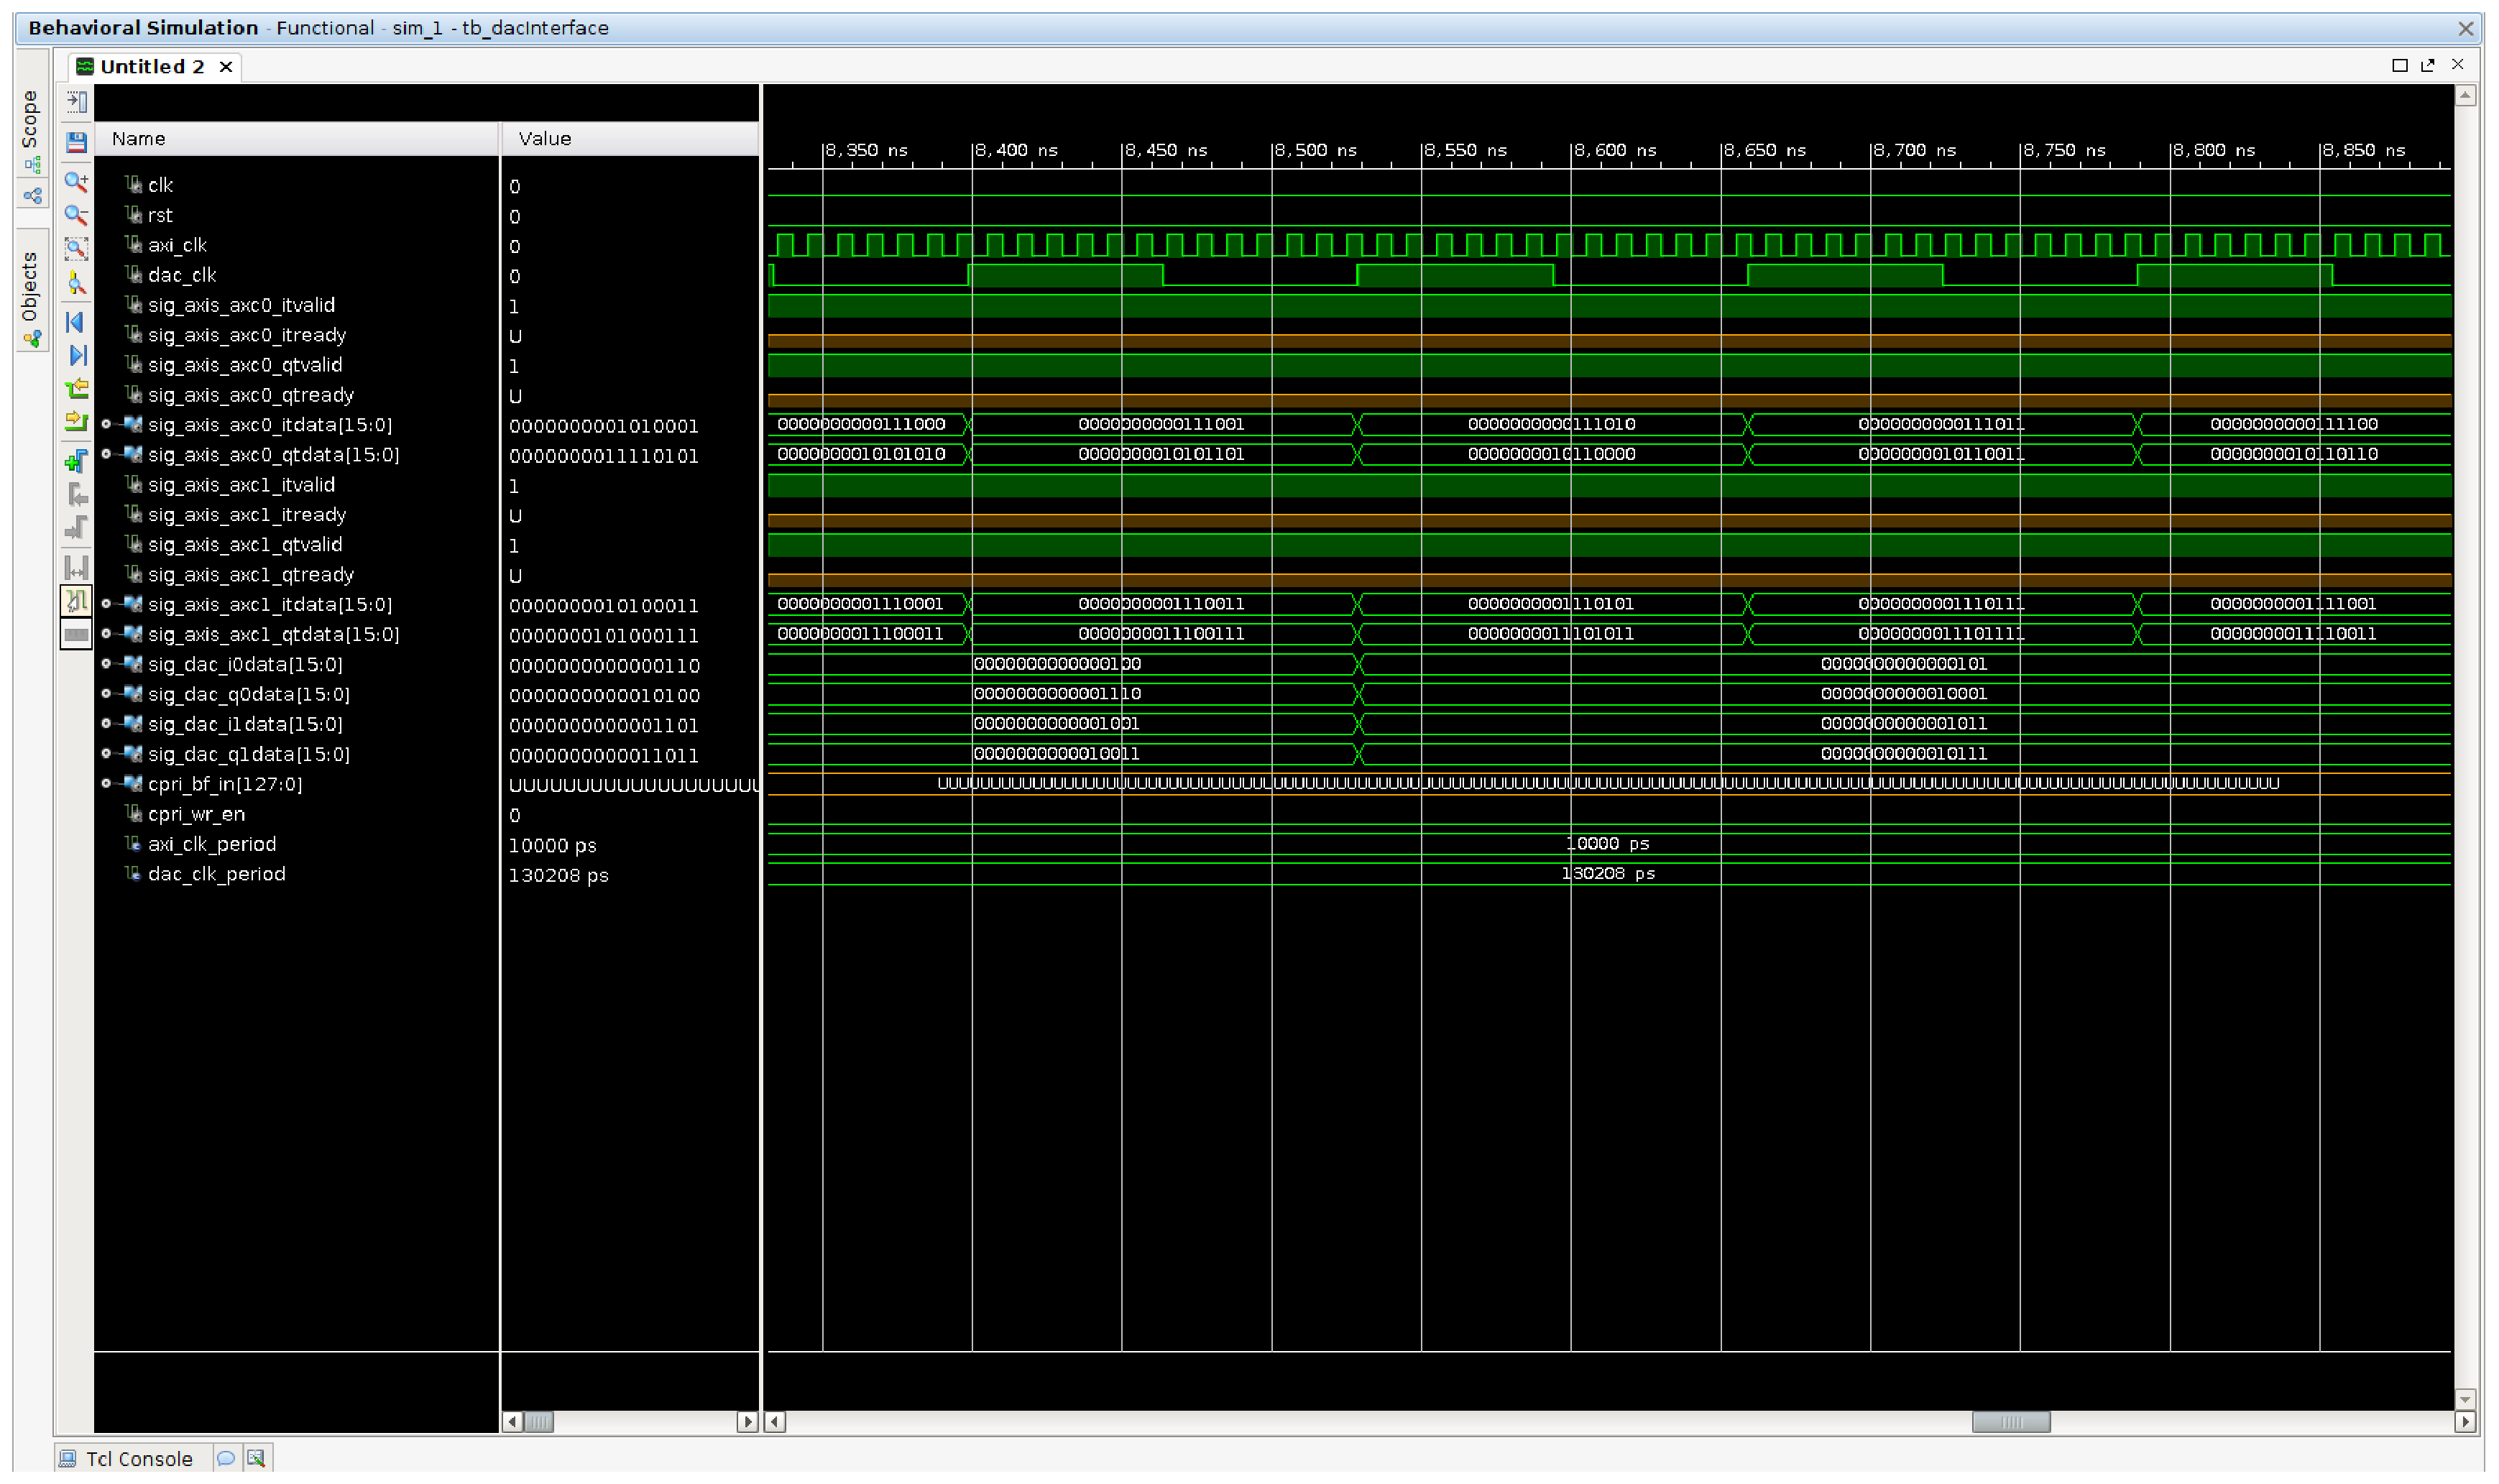
\includegraphics[width=0.95\textwidth]{./figures/dacInterface}
    \caption{ Step 2: DAC Interface Block Simulation
    \label{fig:simdac}}
\end{figure}

\begin{figure}[htbp]
    \centering
    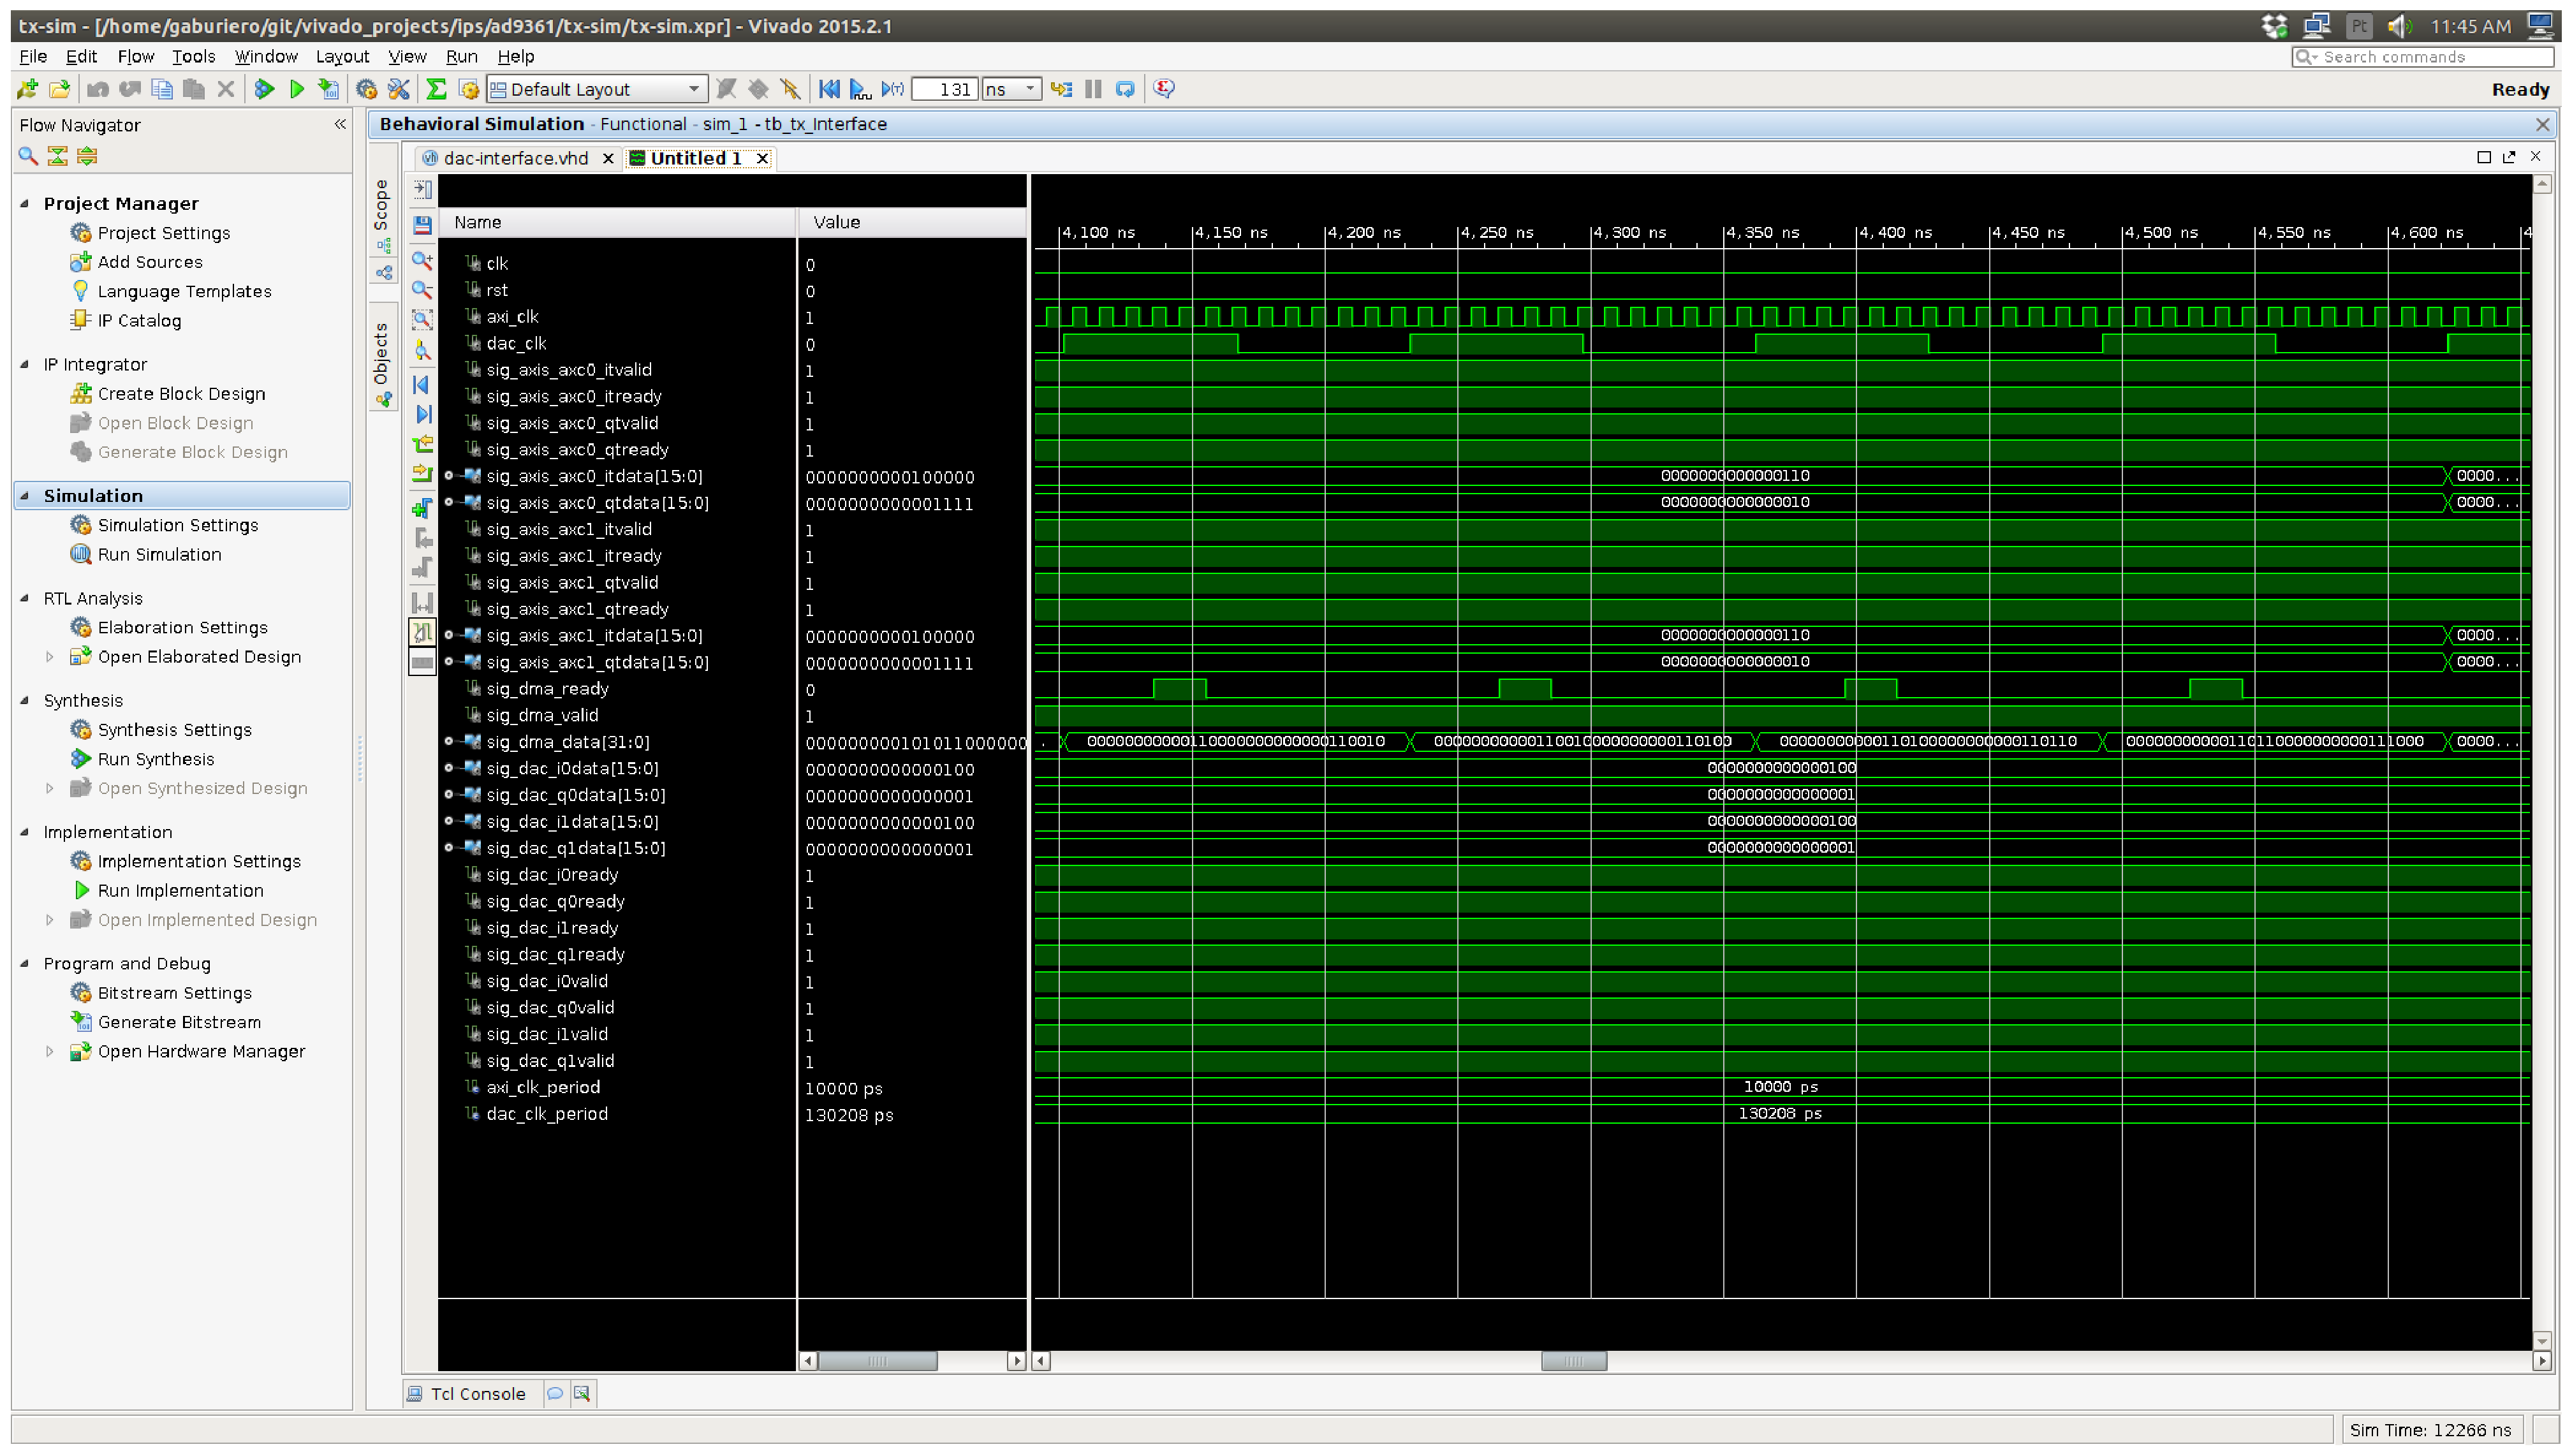
\includegraphics[width=0.95\textwidth]{./figures/txInterface}
    \caption{ Step 3: Transmitting Interface Block Simulation
    \label{fig:simtxif}}
\end{figure}

\subsection{Receive (ADC) Interface Simulation}

As stated before on chapter \ref{chap:implementation} in the section \ref{impl:setup},
the DAC interface is simple beacause the data input is already limited by the DAC
clock, so there is no need to make a bottleneck like in the DAC interface.\\

In the figure \ref{fig:simdac} it is possible to see the output and wave diagram
in the simulation window.

\begin{figure}[htbp]
    \centering
    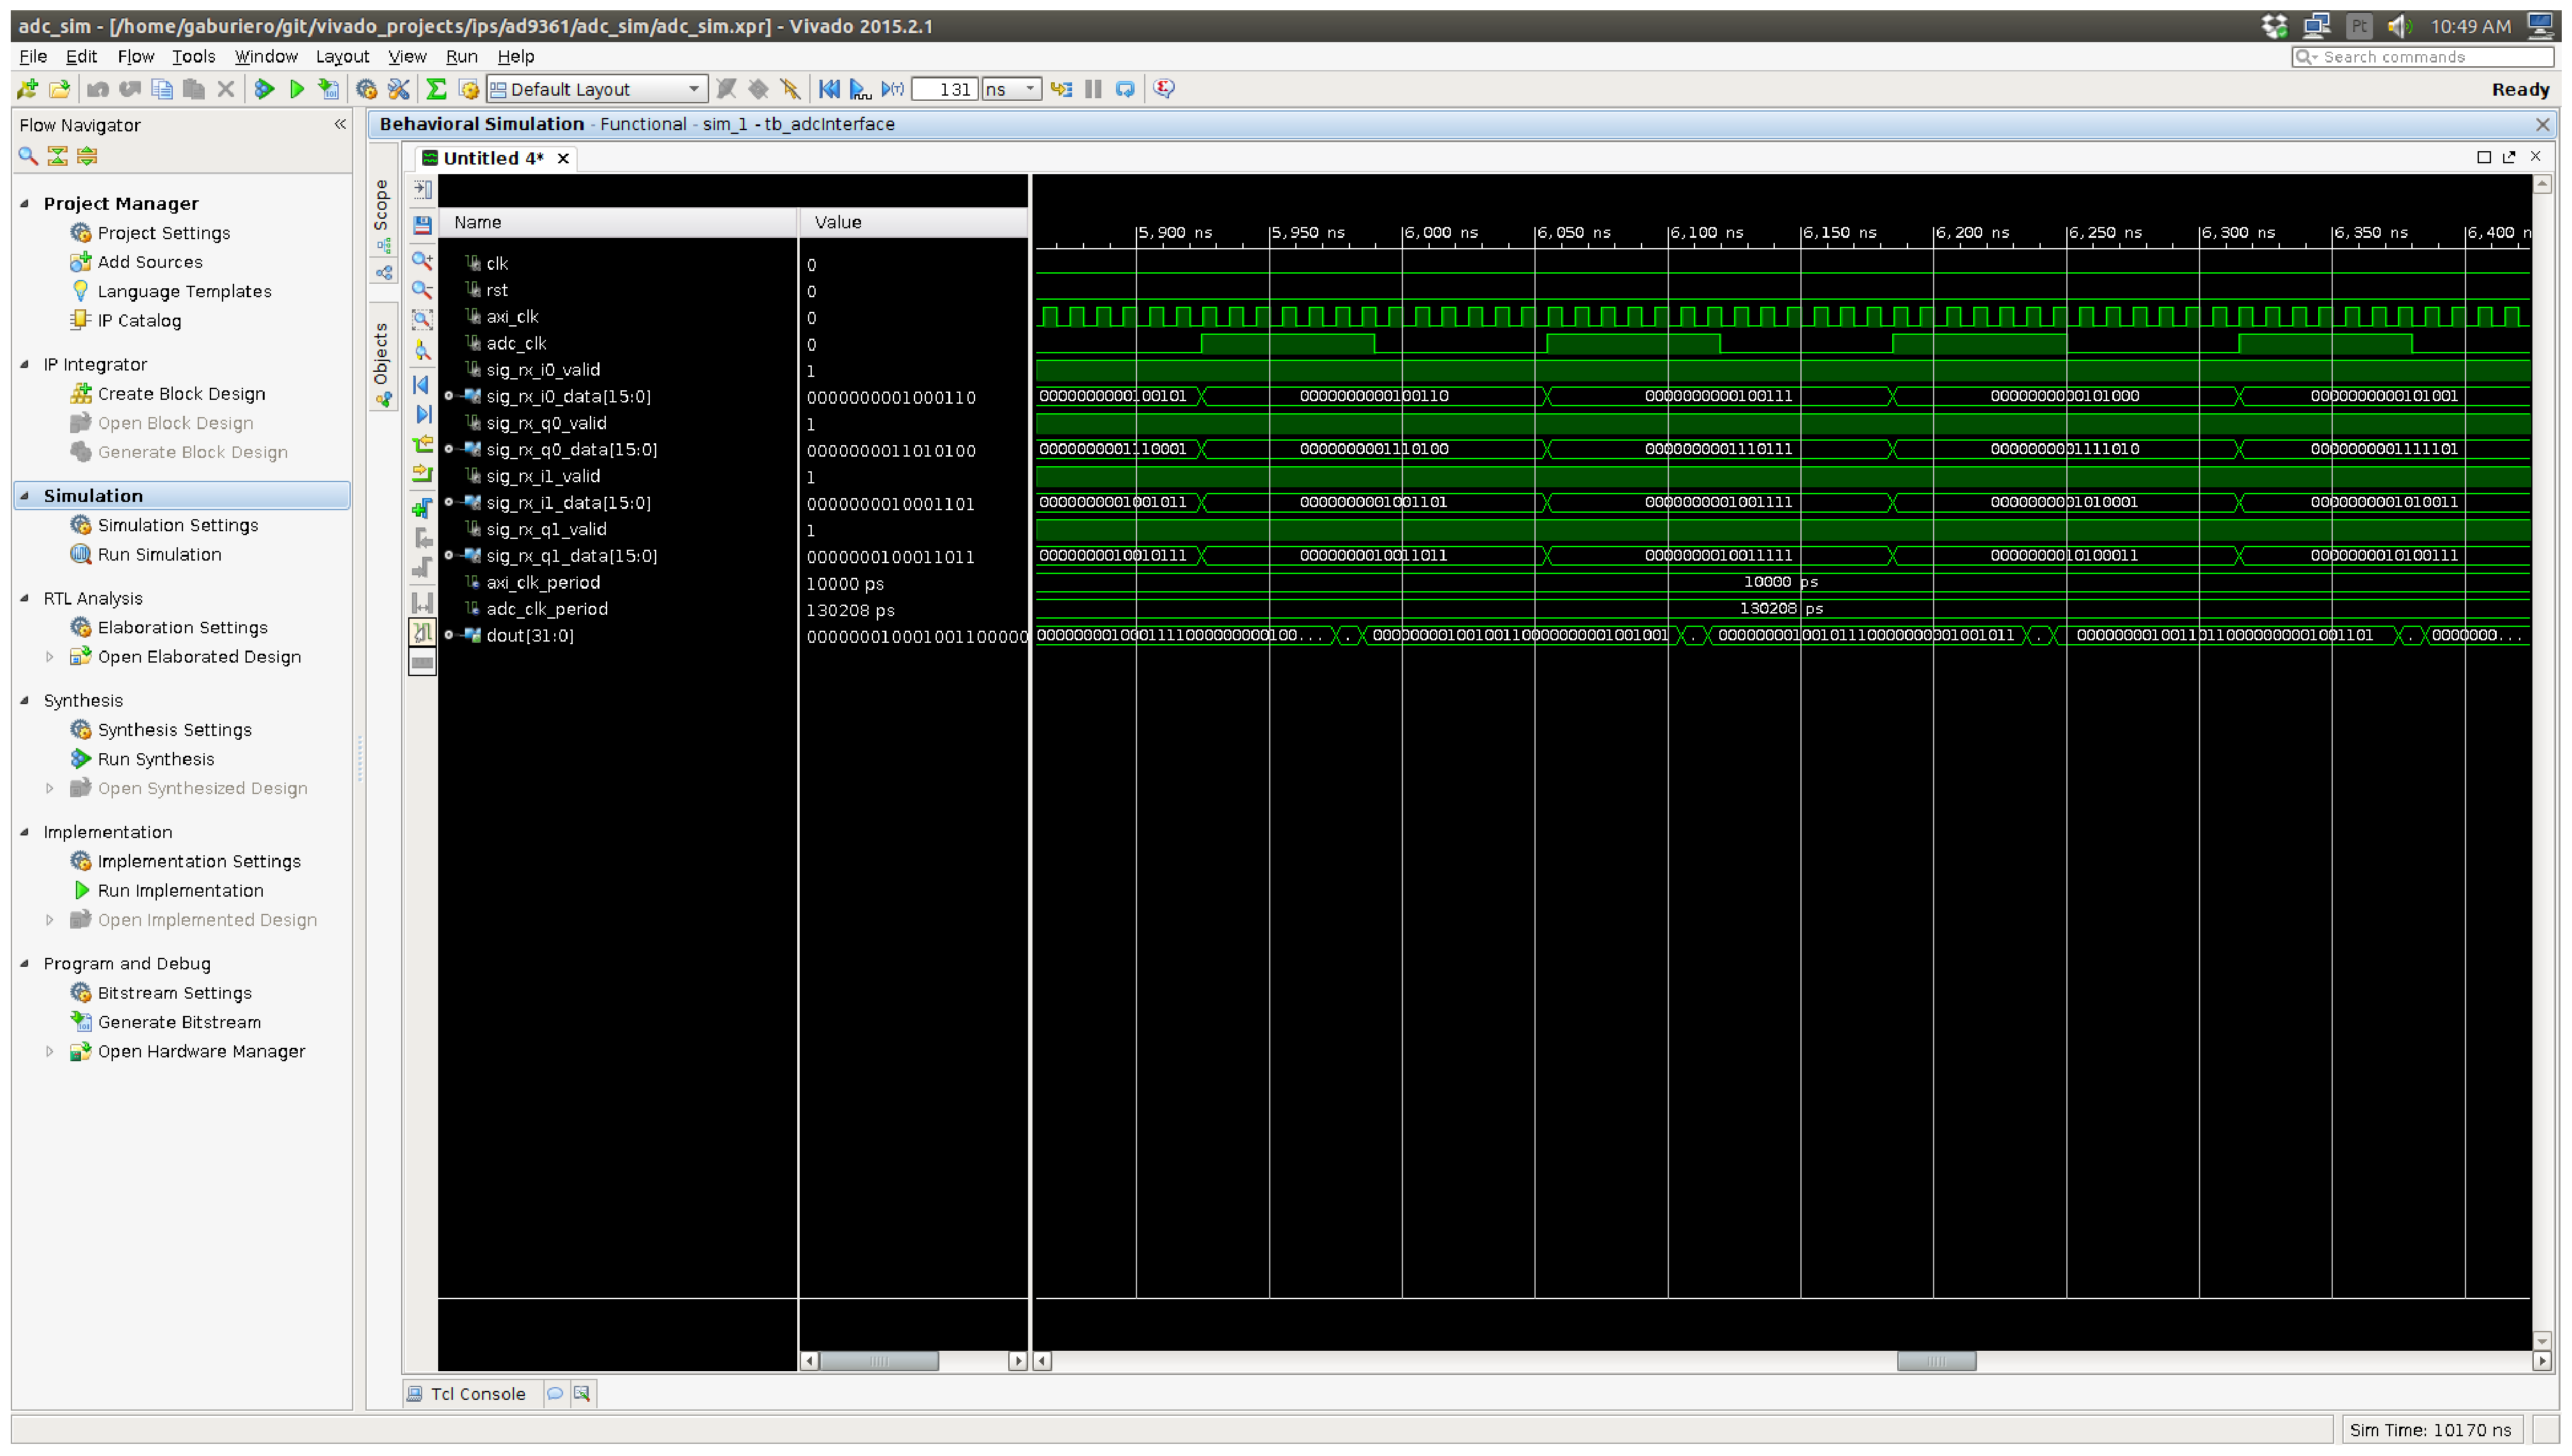
\includegraphics[width=0.95\textwidth]{./figures/adcInterface}
    \caption{ ADC Interface Block Simulation
    \label{fig:simadc}}
\end{figure}

\section{Transmission Tests (DAC)}
\label{result:dac}

\section{Reception Tests (ADC)}
\label{result:adc}
